\documentclass{article} % For LaTeX2e
\usepackage{nips14submit_e,times}
\usepackage{hyperref}
\usepackage{url}
\usepackage{amsmath}
\usepackage{amssymb}
\usepackage{amsthm}
\usepackage{mathtools,enumitem}
\usepackage{algorithm}
\usepackage{algorithmic}
\usepackage{subcaption}
%\documentstyle[nips14submit_09,times,art10]{article} % For LaTeX 2.09

\usepackage{tikz}
\usepackage{cite}

% Math operators
\newcommand{\scal}[2]{\left\langle #1 , #2 \right\rangle}
\DeclareMathOperator{\IR}{\mathbb{R}}
\DeclareMathOperator*{\argmin}{argmin}
\DeclareMathOperator{\One}{\mathbbm{1}}
\DeclareMathOperator{\Ccal}{\mathcal{C}}
\DeclareMathOperator{\logsumexp}{logsumexp}
\DeclareMathOperator{\diag}{diag}
\DeclareMathOperator{\KL}{KL}
\newcommand{\norm}[1]{\left\lVert #1 \right\rVert}
\renewcommand{\epsilon}{\varepsilon}

\theoremstyle{plain}
\newtheorem{theorem}{Theorem}
\newtheorem{proposition}{Proposition}
\newtheorem{lemma}{Lemma}
\newtheorem{corollary}{Corollary}

\theoremstyle{definition}
\newtheorem{definition}{Definition}

\theoremstyle{remark}
\newtheorem{remark}{Remark}
\newtheorem{example}{Example}


\title{Overrelaxed Sinkhorn--Knopp Algorithm for Regularized Optimal Transport}

%
\author{
Alexis THIBAULT\\
\'Ecole Normale Sup\'erieure\\
Paris, France\\
\texttt{alexis.thibault@ens.fr}
 \And
L\'ena\"ic CHIZAT\\
\'Ecole Normale Sup\'erieure\\ Paris Dauphine (PSL research University)\\
Paris, France\\
\texttt{lenaic.chizat@ens.fr}
 \AND
Charles DOSSAL\\
INSA Toulouse\\
Institut de Math\'ematiques de Toulouse\\
Toulouse,  France\\
\texttt{dossal@insa-toulouse.fr}
\And 
Nicolas PAPADAKIS\\
CNRS, Institut de Math\'ematiques de Bordeaux\\
Talence, France\\
\texttt{nicolas.papadakis@math.u-bordeaux.fr}
} 
% The \author macro works with any number of authors. There are two commands
% used to separate the names and addresses of multiple authors: \And and \AND.
%
% Using \And between authors leaves it to \LaTeX{} to determine where to break
% the lines. Using \AND forces a linebreak at that point. So, if \LaTeX{}
% puts 3 of 4 authors names on the first line, and the last on the second
% line, try using \AND instead of \And before the third author name.

\newcommand{\fix}{\marginpar{FIX}}
\newcommand{\new}{\marginpar{NEW}}

\nipsfinalcopy % Uncomment for camera-ready version

\begin{document}


\maketitle

\begin{abstract}
This article describes a method for quickly computing the solution to the regularized optimal transport problem. It generalizes and improves upon the widely-used iterative Bregman projections algorithm (or Sinkhorn--Knopp algorithm). 
The idea is to overrelax the Bregman projection operators, allowing for faster convergence. In practice this corresponds to elevating the diagonal scaling factors to a given power, at each step of the algorithm.
We propose a simple method for establishing global convergence by ensuring the decrease of a Lyapunov function at each step.
An adaptive choice of overrelaxation parameter based on the Lyapunov function is constructed.
We also suggest a heuristic to choose a suitable asymptotic over-relaxation parameter, based on a local convergence analysis. Our numerical experiments show a gain in convergence speed by an order of magnitude in certain regimes.
\end{abstract}

\section{Introduction}
Optimal Transport (OT) is an efficient and flexible tool to compare two probability distributions which has been popularized in the computer vision community in the context of discrete histograms \cite{Rubner2000}. The introduction of entropic regularization in \cite{cuturi13} has made possible the use of the fast Sinkhorn--Knopp algorithm \cite{sinkhorn64}   scaling with high dimensional data. 
Regularized optimal transport have thus been intensively used  in  Machine Learning with applications such as   Geodesic PCA \cite{seguy2015principal}, domain adaptation \cite{2015arXiv150700504C}, data fitting \cite{2015arXiv150605439F},  training of Boltzmann Machine \cite{NIPS2016_6248}  or dictionary learning \cite{Rolet2016,2017arXiv170801955S}.

The computation of optimal transport between two data relies on the estimation of an optimal transport matrix, the entries of which represent the quantity of mass transported between  data locations. 
Regularization of optimal transport with strictly convex regularizers \cite{cuturi13, dessein2016}  nevertheless involves a spreading of the mass. Hence, for particular purposes such as color interpolation \cite{Rabin2014} or gradient flow \cite{2016arXiv160705816C}, it is  necessary  to consider very small regularization of the problem.
In this setting,  the regularized transport problem can be ill-conditioned and Sinkhorn's algorithm converges slowly. This is the issue  we want to tackle here.
Before going into further details, we now briefly introduce the main notations and concepts used all along this article.

 
\subsection{Discrete optimal transport}
We consider two discrete probability measures $\mu^k \in \IR_{+*}^{n_k}$.
Let us define the two following linear operators
\begin{align*}
A_1 &: \begin{cases}
\IR^{n_1 n_2} \rightarrow \IR^{n_1} \\
(A_1 x)_i = \sum_j x_{i,j}
\end{cases} &
A_2 &: \begin{cases}
\IR^{n_1 n_2} \rightarrow \IR^{n_2}\\
(A_2 x)_j = \sum_i x_{i,j},
\end{cases}
\end{align*}
as well as the affine constraint sets
\begin{align*}
\Ccal_k &= \left\{ \gamma\in\IR^{n_1 n_2} \mid A_k \gamma = \mu^k \right\}.
\end{align*}
Given a cost matrix $c$, where $c_{ij}$ represents the cost of moving mass $\mu^1_i$ to $\mu^2_j$,  the optimal transport problem corresponds to the estimation of an optimal transport matrix $\gamma$ solution of:
$$\min_{\gamma\in\Ccal_1\cap \Ccal_2\cap \IR^{n_1 n_2}_+} \langle c,\gamma\rangle:=\sum_{i,j}c_{i,j}\gamma_{i,j}.$$
This is a linear programming problem whose resolution becomes intractable for large problems.

\subsection{Regularized optimal transport}

In \cite{cuturi13}, it has been proposed to regularize this problem by adding a strictly convex entropy regularization:
\begin{equation}\label{ROT}
\min_{\gamma\in\Ccal_1\cap \Ccal_2\cap \IR^{n_1 n_2}_{+}}K^\epsilon(\gamma) \coloneqq \scal{c}{\gamma} 
+ \epsilon \KL(\gamma,\mathbf{1})
,\end{equation}
with $\epsilon>0$, $\mathbf{1}$ is the matrix of size $n_1\times n_2$ full of ones and the Kullback-Leibler divergence is
\begin{equation}\label{KL}
\KL(\gamma,\xi) = \sum_{i,j} \gamma_{i,j} \left( \log \left( \frac{\gamma_{i,j}}{\xi_{i,j}} \right) -1  \right) + \sum_{i,j} \xi_{i,j}
\end{equation}
with the convention $0 \log 0= 0$. It was shown in \cite{benamou15}  that the regularized optimal transport matrix $\gamma^*$, which is the unique minimizer of problem \eqref{ROT},  is the Bregman projection of $\gamma^0 = e^{-c/\epsilon}$ (here and in the sequel, exponentiation is meant entrywise) onto $\Ccal_1 \cap \Ccal_2$:
\begin{equation}\label{eq:reg_ot_pb}
\gamma^* = \argmin_{\Ccal_1 \cap \Ccal_2} K^\epsilon(\gamma)= P_{\Ccal_1 \cap \Ccal_2} (e^{-c/\epsilon}),
\end{equation}
where $P_{\Ccal}$ is the  Bregman projection onto $\Ccal$ defined as
\[
P_{\Ccal}(\xi) \coloneqq \argmin_{\gamma \in \Ccal} \KL(\gamma,\xi).
\]



\subsection{Sinkhorn--Knopp algorithm}
Iterative Bregman projections onto $\Ccal_1$ and $\Ccal_2$ converge to a point in the intersection $\Ccal_1 \cap \Ccal_2$ \cite{bregman67}. Hence, the so-called Sinkhorn--Knopp algorithm (SK) \cite{sinkhorn64} that performs alternate Bregman projections, can be considered to compute the regularized  transport matrix:
\begin{align*}
\gamma^0 &= e^{-c/\epsilon} &
\gamma^{l+1} = P_{\Ccal_2}(P_{\Ccal_1}(\gamma^l)),
\end{align*}
and we have 
$\lim_{l\rightarrow +\infty} \gamma^l = P_{\Ccal_1 \cap \Ccal_2}(\gamma^0) = \gamma^*.$
%
In the discrete setting, these projections correspond to diagonal scalings of the input:
\begin{align}\label{scaling}
P_{\Ccal_1}(\gamma) &= \diag(a) \gamma &\text{with}\quad
a &=  {\mu^1}\oslash{A_1 \gamma} \\
P_{\Ccal_2}(\gamma) &= \gamma \diag(b) &\text{with}\quad
b &= {\mu^2}\oslash{A_2 \gamma}\nonumber
\end{align}
where $\oslash$ is the pointwise division. 
To compute numerically the solution one simply has to store $(a^l, b^l)\in\IR^{n_1}\times \IR^{n_2}$ and to iterate
\begin{align*}
a^{l+1} &= {\mu^1}\oslash{\gamma^0 b^l} &
b^{l+1} &= {\mu^2}\oslash{^t \gamma^0 a^{l+1}} .
\end{align*}
We then have $\gamma^l = \diag(a^l) \gamma^0 \diag(b^l).$ 

Another way to interpret the SK algorithm is as an alternate maximization algorithm on the dual of the regularized optimal transport problem. The dual problem of \eqref{ROT} is
\begin{equation}\label{DROT}
\max_{\substack{\alpha\in \IR^n\\\beta\in \IR^m}}\; E(\alpha,\beta) \coloneqq \langle \alpha,\mu^1\rangle+\langle \beta,\mu^2\rangle-\epsilon\sum_{i,j}e^{(\alpha_i+\beta_j-c_{i,j})/\epsilon}.
\end{equation}
The function $E$ is concave, continuously differentiable and admits a maximizer, so alternate maximization converges and we recover, for $a_i=e^{\alpha_i/\epsilon}$, $b_j=e^{\beta_j/\epsilon}$ and $\gamma^0_{i,j}=e^{-c_{i,j}/\epsilon}$:
\begin{align*}
a^{l+1} &= {\mu^1}\oslash{\gamma^0 b^l} &
b^{l+1} &= {\mu^2}\oslash{^t \gamma^0 a^{l+1}} 
\end{align*}



Efficient parallel computations can be considered \cite{cuturi13} and one can even reach real-time computation for large scale problem for certain class of cost matrices $c$ \cite{Solomon2015}. 
For small values of the parameter $\epsilon$, numerical issues can arise and a stabilization of the algorithm is necessary \cite{2016arXiv160705816C}.
The convergence of the process can nevertheless be very slow when $\epsilon$ is small.

\subsection{Overview and contributions}
In this paper, we consider an overrelaxation scheme designed to accelerate the Sinkhorn--Knopp algorithm. We first present and show the convergence of our algorithm in section 2. In section 3, we analyze the local convergence rate of the algorithm to justify the acceleration.
We finally demonstrate numerically  in Section 4 the good behavior of our method, where larger accelerations are observed for decreasing values of $\epsilon$.

\subsection{Related works }
The introduction of relaxation variables through heavy ball approaches \cite{POLYAK19641} has recently gained in popularity  to speed up the convergence of algorithms optimizing convex \cite{2014arXiv1412.7457G} or non convex \cite{Zavriev1993,2016arXiv160609070O} problems. Such schemes have also been empirically considered to accelerate the SK algorithm  in \cite{peyre2016quantum,2017arXiv170801955S}. The convergence of these algorithms is nevertheless not studied yet in the context of regularized optimal transport.


\section{Overrelaxed Sinkhorn--Knopp algorithm}

As illustrated in Figure \ref{alternate_projections} (a-b), the SK algorithm, that  performs alternate Bregman projections onto the affine sets $\Ccal_1$ and $\Ccal_2$, can be very slow when $\epsilon\to 0$. The idea developped in this paper is to perform overrelaxed projections in order to accelerate the process, as displayed in Figure \ref{alternate_projections} (c).

\begin{figure}[ht!]
\centering
\begin{minipage}[b]{.33\linewidth}
   \centering
   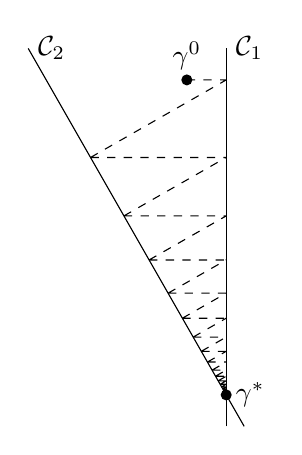
\begin{tikzpicture}
\fill (-0.500000,4.000000) circle (2pt) node[above] (gamma0) {$\gamma^0$};
\fill (0,0) circle (2pt) node[right] {$\gamma^*$};
\draw[dashed] (-0.500000,4.000000) -- (0.000000,4.000000)
(-1.723077,3.015385) -- (0.000000,4.000000)
(-1.723077,3.015385) -- (0.000000,3.015385)
(-1.298935,2.273136) -- (0.000000,3.015385)
(-1.298935,2.273136) -- (0.000000,2.273136)
(-0.979197,1.713595) -- (0.000000,2.273136)
(-0.979197,1.713595) -- (0.000000,1.713595)
(-0.738164,1.291787) -- (0.000000,1.713595)
(-0.738164,1.291787) -- (0.000000,1.291787)
(-0.556462,0.973809) -- (0.000000,1.291787)
(-0.556462,0.973809) -- (0.000000,0.973809)
(-0.419487,0.734102) -- (0.000000,0.973809)
(-0.419487,0.734102) -- (0.000000,0.734102)
(-0.316228,0.553400) -- (0.000000,0.734102)
(-0.316228,0.553400) -- (0.000000,0.553400)
(-0.238388,0.417178) -- (0.000000,0.553400)
(-0.238388,0.417178) -- (0.000000,0.417178)
(-0.179708,0.314488) -- (0.000000,0.417178)
(-0.179708,0.314488) -- (0.000000,0.314488)
(-0.135472,0.237076) -- (0.000000,0.314488)
(-0.135472,0.237076) -- (0.000000,0.237076)
(-0.102125,0.178719) -- (0.000000,0.237076)
(-0.102125,0.178719) -- (0.000000,0.178719)
(-0.076987,0.134726) -- (0.000000,0.178719)
(-0.076987,0.134726) -- (0.000000,0.134726)
(-0.058036,0.101563) -- (0.000000,0.134726)
(-0.058036,0.101563) -- (0.000000,0.101563)
(-0.043750,0.076563) -- (0.000000,0.101563)
(-0.043750,0.076563) -- (0.000000,0.076563)
(-0.032981,0.057717) -- (0.000000,0.076563)
(-0.032981,0.057717) -- (0.000000,0.057717)
(-0.024863,0.043509) -- (0.000000,0.057717)
(-0.024863,0.043509) -- (0.000000,0.043509)
(-0.018743,0.032799) -- (0.000000,0.043509)
(-0.018743,0.032799) -- (0.000000,0.032799)
(-0.014129,0.024726) -- (0.000000,0.032799)
(-0.014129,0.024726) -- (0.000000,0.024726)
(-0.010651,0.018639) -- (0.000000,0.024726)
(-0.010651,0.018639) -- (0.000000,0.018639)
(-0.008029,0.014051) -- (0.000000,0.018639)
(-0.008029,0.014051) -- (0.000000,0.014051)
(-0.006053,0.010592) -- (0.000000,0.014051)
(-0.006053,0.010592) -- (0.000000,0.010592)
(-0.004563,0.007985) -- (0.000000,0.010592)
(-0.004563,0.007985) -- (0.000000,0.007985)
(-0.003440,0.006020) -- (0.000000,0.007985)
(-0.003440,0.006020) -- (0.000000,0.006020)
(-0.002593,0.004538) -- (0.000000,0.006020)
(-0.002593,0.004538) -- (0.000000,0.004538)
(-0.001955,0.003421) -- (0.000000,0.004538)
(-0.001955,0.003421) -- (0.000000,0.003421)
(-0.001474,0.002579) -- (0.000000,0.003421)
(-0.001474,0.002579) -- (0.000000,0.002579)
(-0.001111,0.001944) -- (0.000000,0.002579)
(-0.001111,0.001944) -- (0.000000,0.001944)
(-0.000837,0.001465) -- (0.000000,0.001944)
(-0.000837,0.001465) -- (0.000000,0.001465)
(-0.000631,0.001105) -- (0.000000,0.001465)
(-0.000631,0.001105) -- (0.000000,0.001105)
(-0.000476,0.000833) -- (0.000000,0.001105)
(-0.000476,0.000833) -- (0.000000,0.000833)
(-0.000359,0.000628) -- (0.000000,0.000833)
(-0.000359,0.000628) -- (0.000000,0.000628)
(-0.000270,0.000473) -- (0.000000,0.000628)
(-0.000270,0.000473) -- (0.000000,0.000473)
(-0.000204,0.000357) -- (0.000000,0.000473)
(-0.000204,0.000357) -- (0.000000,0.000357)
(-0.000154,0.000269) -- (0.000000,0.000357)
(-0.000154,0.000269) -- (0.000000,0.000269)
(-0.000116,0.000203) -- (0.000000,0.000269)
(-0.000116,0.000203) -- (0.000000,0.000203)
(-0.000087,0.000153) -- (0.000000,0.000203)
(-0.000087,0.000153) -- (0.000000,0.000153)
(-0.000066,0.000115) -- (0.000000,0.000153)
(-0.000066,0.000115) -- (0.000000,0.000115)
(-0.000050,0.000087) -- (0.000000,0.000115)
(-0.000050,0.000087) -- (0.000000,0.000087)
(-0.000037,0.000065) -- (0.000000,0.000087)
(-0.000037,0.000065) -- (0.000000,0.000065)
(-0.000028,0.000049) -- (0.000000,0.000065)
(-0.000028,0.000049) -- (0.000000,0.000049)
(-0.000021,0.000037) -- (0.000000,0.000049)
(-0.000021,0.000037) -- (0.000000,0.000037)
(-0.000016,0.000028) -- (0.000000,0.000037)
(-0.000016,0.000028) -- (0.000000,0.000028)
(-0.000012,0.000021) -- (0.000000,0.000028)
(-0.000012,0.000021) -- (0.000000,0.000021)
(-0.000009,0.000016) -- (0.000000,0.000021)
(-0.000009,0.000016) -- (0.000000,0.000016)
(-0.000007,0.000012) -- (0.000000,0.000016)
(-0.000007,0.000012) -- (0.000000,0.000012)
(-0.000005,0.000009) -- (0.000000,0.000012)
(-0.000005,0.000009) -- (0.000000,0.000009)
(-0.000004,0.000007) -- (0.000000,0.000009)
(-0.000004,0.000007) -- (0.000000,0.000007)
(-0.000003,0.000005) -- (0.000000,0.000007)
(-0.000003,0.000005) -- (0.000000,0.000005)
(-0.000002,0.000004) -- (0.000000,0.000005)
(-0.000002,0.000004) -- (0.000000,0.000004)
(-0.000002,0.000003) -- (0.000000,0.000004)
(-0.000002,0.000003) -- (0.000000,0.000003)
(-0.000001,0.000002) -- (0.000000,0.000003)
(-0.000001,0.000002) -- (0.000000,0.000002)
(-0.000001,0.000002) -- (0.000000,0.000002)
(-0.000001,0.000002) -- (0.000000,0.000002)
(-0.000001,0.000001) -- (0.000000,0.000002)
(-0.000001,0.000001) -- (0.000000,0.000001)
(-0.000001,0.000001) -- (0.000000,0.000001)
(-0.000001,0.000001) -- (0.000000,0.000001)
(-0.000000,0.000001) -- (0.000000,0.000001)
(-0.000000,0.000001) -- (0.000000,0.000001)
(-0.000000,0.000001) -- (0.000000,0.000001)
(-0.000000,0.000001) -- (0.000000,0.000001)
(-0.000000,0.000000) -- (0.000000,0.000001)
(-0.000000,0.000000) -- (0.000000,0.000000)
(-0.000000,0.000000) -- (0.000000,0.000000)
(-0.000000,0.000000) -- (0.000000,0.000000)
(-0.000000,0.000000) -- (0.000000,0.000000)
(-0.000000,0.000000) -- (0.000000,0.000000)
(-0.000000,0.000000) -- (0.000000,0.000000)
(-0.000000,0.000000) -- (0.000000,0.000000)
(-0.000000,0.000000) -- (0.000000,0.000000)
(-0.000000,0.000000) -- (0.000000,0.000000)
(-0.000000,0.000000) -- (0.000000,0.000000)
(-0.000000,0.000000) -- (0.000000,0.000000)
(-0.000000,0.000000) -- (0.000000,0.000000)
(-0.000000,0.000000) -- (0.000000,0.000000)
(-0.000000,0.000000) -- (0.000000,0.000000)
(-0.000000,0.000000) -- (0.000000,0.000000)
(-0.000000,0.000000) -- (0.000000,0.000000)
(-0.000000,0.000000) -- (0.000000,0.000000)
(-0.000000,0.000000) -- (0.000000,0.000000)
(-0.000000,0.000000) -- (0.000000,0.000000)
(-0.000000,0.000000) -- (0.000000,0.000000)
(-0.000000,0.000000) -- (0.000000,0.000000)
(-0.000000,0.000000) -- (0.000000,0.000000)
(-0.000000,0.000000) -- (0.000000,0.000000)
(-0.000000,0.000000) -- (0.000000,0.000000)
(-0.000000,0.000000) -- (0.000000,0.000000)
(-0.000000,0.000000) -- (0.000000,0.000000)
(-0.000000,0.000000) -- (0.000000,0.000000)
(-0.000000,0.000000) -- (0.000000,0.000000)
(-0.000000,0.000000) -- (0.000000,0.000000)
(-0.000000,0.000000) -- (0.000000,0.000000)
(-0.000000,0.000000) -- (0.000000,0.000000)
(-0.000000,0.000000) -- (0.000000,0.000000)
(-0.000000,0.000000) -- (0.000000,0.000000)
(-0.000000,0.000000) -- (0.000000,0.000000)
(-0.000000,0.000000) -- (0.000000,0.000000)
(-0.000000,0.000000) -- (0.000000,0.000000)
(-0.000000,0.000000) -- (0.000000,0.000000)
(-0.000000,0.000000) -- (0.000000,0.000000)
(-0.000000,0.000000) -- (0.000000,0.000000)
(-0.000000,0.000000) -- (0.000000,0.000000)
(-0.000000,0.000000) -- (0.000000,0.000000)
(-0.000000,0.000000) -- (0.000000,0.000000)
(-0.000000,0.000000) -- (0.000000,0.000000)
(-0.000000,0.000000) -- (0.000000,0.000000)
(-0.000000,0.000000) -- (0.000000,0.000000)
(-0.000000,0.000000) -- (0.000000,0.000000)
(-0.000000,0.000000) -- (0.000000,0.000000)
(-0.000000,0.000000) -- (0.000000,0.000000)
(-0.000000,0.000000) -- (0.000000,0.000000)
(-0.000000,0.000000) -- (0.000000,0.000000)
(-0.000000,0.000000) -- (0.000000,0.000000)
(-0.000000,0.000000) -- (0.000000,0.000000)
(-0.000000,0.000000) -- (0.000000,0.000000)
(-0.000000,0.000000) -- (0.000000,0.000000)
(-0.000000,0.000000) -- (0.000000,0.000000)
(-0.000000,0.000000) -- (0.000000,0.000000)
(-0.000000,0.000000) -- (0.000000,0.000000)
(-0.000000,0.000000) -- (0.000000,0.000000)
(-0.000000,0.000000) -- (0.000000,0.000000)
(-0.000000,0.000000) -- (0.000000,0.000000)
(-0.000000,0.000000) -- (0.000000,0.000000)
(-0.000000,0.000000) -- (0.000000,0.000000)
(-0.000000,0.000000) -- (0.000000,0.000000)
(-0.000000,0.000000) -- (0.000000,0.000000)
(-0.000000,0.000000) -- (0.000000,0.000000)
(-0.000000,0.000000) -- (0.000000,0.000000)
(-0.000000,0.000000) -- (0.000000,0.000000)
(-0.000000,0.000000) -- (0.000000,0.000000)
(-0.000000,0.000000) -- (0.000000,0.000000)
(-0.000000,0.000000) -- (0.000000,0.000000)
(-0.000000,0.000000) -- (0.000000,0.000000)
(-0.000000,0.000000) -- (0.000000,0.000000)
(-0.000000,0.000000) -- (0.000000,0.000000)
(-0.000000,0.000000) -- (0.000000,0.000000)
(-0.000000,0.000000) -- (0.000000,0.000000)
(-0.000000,0.000000) -- (0.000000,0.000000)
(-0.000000,0.000000) -- (0.000000,0.000000)
(-0.000000,0.000000) -- (0.000000,0.000000)
(-0.000000,0.000000) -- (0.000000,0.000000)
(-0.000000,0.000000) -- (0.000000,0.000000)
(-0.000000,0.000000) -- (0.000000,0.000000)
(-0.000000,0.000000) -- (0.000000,0.000000)
(-0.000000,0.000000) -- (0.000000,0.000000)
(-0.000000,0.000000) -- (0.000000,0.000000)
(-0.000000,0.000000) -- (0.000000,0.000000)
(-0.000000,0.000000) -- (0.000000,0.000000)
;
\draw (-0.000000,-0.400000) -- (0.000000,4.400000) node[right] {$\mathcal{C}_1$};
\draw (0.228571,-0.400000) -- (-2.514286,4.400000) node[right] {$\mathcal{C}_2$};
\end{tikzpicture}

                    \subcaption{}\label{fig:schema_a}
\end{minipage}%
\begin{minipage}[b]{.33\linewidth}
   \centering
   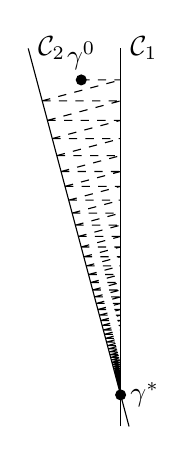
\begin{tikzpicture}
\fill (-0.500000,4.000000) circle (2pt) node[above] (gamma0) {$\gamma^0$};
\fill (0,0) circle (2pt) node[right] {$\gamma^*$};
\draw[dashed] (-0.500000,4.000000) -- (0.000000,4.000000)
(-0.995851,3.734440) -- (0.000000,4.000000)
(-0.995851,3.734440) -- (0.000000,3.734440)
(-0.929736,3.486510) -- (0.000000,3.734440)
(-0.929736,3.486510) -- (0.000000,3.486510)
(-0.868011,3.255041) -- (0.000000,3.486510)
(-0.868011,3.255041) -- (0.000000,3.255041)
(-0.810384,3.038938) -- (0.000000,3.255041)
(-0.810384,3.038938) -- (0.000000,3.038938)
(-0.756582,2.837183) -- (0.000000,3.038938)
(-0.756582,2.837183) -- (0.000000,2.837183)
(-0.706353,2.648822) -- (0.000000,2.837183)
(-0.706353,2.648822) -- (0.000000,2.648822)
(-0.659458,2.472967) -- (0.000000,2.648822)
(-0.659458,2.472967) -- (0.000000,2.472967)
(-0.615676,2.308787) -- (0.000000,2.472967)
(-0.615676,2.308787) -- (0.000000,2.308787)
(-0.574802,2.155506) -- (0.000000,2.308787)
(-0.574802,2.155506) -- (0.000000,2.155506)
(-0.536641,2.012402) -- (0.000000,2.155506)
(-0.536641,2.012402) -- (0.000000,2.012402)
(-0.501013,1.878799) -- (0.000000,2.012402)
(-0.501013,1.878799) -- (0.000000,1.878799)
(-0.467751,1.754065) -- (0.000000,1.878799)
(-0.467751,1.754065) -- (0.000000,1.754065)
(-0.436697,1.637613) -- (0.000000,1.754065)
(-0.436697,1.637613) -- (0.000000,1.637613)
(-0.407704,1.528891) -- (0.000000,1.637613)
(-0.407704,1.528891) -- (0.000000,1.528891)
(-0.380637,1.427388) -- (0.000000,1.528891)
(-0.380637,1.427388) -- (0.000000,1.427388)
(-0.355366,1.332624) -- (0.000000,1.427388)
(-0.355366,1.332624) -- (0.000000,1.332624)
(-0.331774,1.244151) -- (0.000000,1.332624)
(-0.331774,1.244151) -- (0.000000,1.244151)
(-0.309747,1.161552) -- (0.000000,1.244151)
(-0.309747,1.161552) -- (0.000000,1.161552)
(-0.289183,1.084436) -- (0.000000,1.161552)
(-0.289183,1.084436) -- (0.000000,1.084436)
(-0.269984,1.012440) -- (0.000000,1.084436)
(-0.269984,1.012440) -- (0.000000,1.012440)
(-0.252060,0.945225) -- (0.000000,1.012440)
(-0.252060,0.945225) -- (0.000000,0.945225)
(-0.235326,0.882471) -- (0.000000,0.945225)
(-0.235326,0.882471) -- (0.000000,0.882471)
(-0.219702,0.823884) -- (0.000000,0.882471)
(-0.219702,0.823884) -- (0.000000,0.823884)
(-0.205116,0.769186) -- (0.000000,0.823884)
(-0.205116,0.769186) -- (0.000000,0.769186)
(-0.191499,0.718120) -- (0.000000,0.769186)
(-0.191499,0.718120) -- (0.000000,0.718120)
(-0.178785,0.670444) -- (0.000000,0.718120)
(-0.178785,0.670444) -- (0.000000,0.670444)
(-0.166915,0.625933) -- (0.000000,0.670444)
(-0.166915,0.625933) -- (0.000000,0.625933)
(-0.155834,0.584377) -- (0.000000,0.625933)
(-0.155834,0.584377) -- (0.000000,0.584377)
(-0.145488,0.545580) -- (0.000000,0.584377)
(-0.145488,0.545580) -- (0.000000,0.545580)
(-0.135829,0.509359) -- (0.000000,0.545580)
(-0.135829,0.509359) -- (0.000000,0.509359)
(-0.126811,0.475543) -- (0.000000,0.509359)
(-0.126811,0.475543) -- (0.000000,0.475543)
(-0.118392,0.443972) -- (0.000000,0.475543)
(-0.118392,0.443972) -- (0.000000,0.443972)
(-0.110532,0.414496) -- (0.000000,0.443972)
(-0.110532,0.414496) -- (0.000000,0.414496)
(-0.103194,0.386978) -- (0.000000,0.414496)
(-0.103194,0.386978) -- (0.000000,0.386978)
(-0.096343,0.361286) -- (0.000000,0.386978)
(-0.096343,0.361286) -- (0.000000,0.361286)
(-0.089947,0.337301) -- (0.000000,0.361286)
(-0.089947,0.337301) -- (0.000000,0.337301)
(-0.083975,0.314907) -- (0.000000,0.337301)
(-0.083975,0.314907) -- (0.000000,0.314907)
(-0.078400,0.294000) -- (0.000000,0.314907)
(-0.078400,0.294000) -- (0.000000,0.294000)
(-0.073195,0.274482) -- (0.000000,0.294000)
(-0.073195,0.274482) -- (0.000000,0.274482)
(-0.068336,0.256259) -- (0.000000,0.274482)
(-0.068336,0.256259) -- (0.000000,0.256259)
(-0.063799,0.239246) -- (0.000000,0.256259)
(-0.063799,0.239246) -- (0.000000,0.239246)
(-0.059563,0.223362) -- (0.000000,0.239246)
(-0.059563,0.223362) -- (0.000000,0.223362)
(-0.055609,0.208533) -- (0.000000,0.223362)
(-0.055609,0.208533) -- (0.000000,0.208533)
(-0.051917,0.194689) -- (0.000000,0.208533)
(-0.051917,0.194689) -- (0.000000,0.194689)
(-0.048470,0.181763) -- (0.000000,0.194689)
(-0.048470,0.181763) -- (0.000000,0.181763)
(-0.045252,0.169696) -- (0.000000,0.181763)
(-0.045252,0.169696) -- (0.000000,0.169696)
(-0.042248,0.158430) -- (0.000000,0.169696)
(-0.042248,0.158430) -- (0.000000,0.158430)
(-0.039443,0.147912) -- (0.000000,0.158430)
(-0.039443,0.147912) -- (0.000000,0.147912)
(-0.036825,0.138092) -- (0.000000,0.147912)
(-0.036825,0.138092) -- (0.000000,0.138092)
(-0.034380,0.128924) -- (0.000000,0.138092)
(-0.034380,0.128924) -- (0.000000,0.128924)
(-0.032097,0.120365) -- (0.000000,0.128924)
(-0.032097,0.120365) -- (0.000000,0.120365)
(-0.029966,0.112374) -- (0.000000,0.120365)
(-0.029966,0.112374) -- (0.000000,0.112374)
(-0.027977,0.104913) -- (0.000000,0.112374)
(-0.027977,0.104913) -- (0.000000,0.104913)
(-0.026119,0.097948) -- (0.000000,0.104913)
(-0.026119,0.097948) -- (0.000000,0.097948)
(-0.024385,0.091445) -- (0.000000,0.097948)
(-0.024385,0.091445) -- (0.000000,0.091445)
(-0.022766,0.085374) -- (0.000000,0.091445)
(-0.022766,0.085374) -- (0.000000,0.085374)
(-0.021255,0.079706) -- (0.000000,0.085374)
(-0.021255,0.079706) -- (0.000000,0.079706)
(-0.019844,0.074415) -- (0.000000,0.079706)
(-0.019844,0.074415) -- (0.000000,0.074415)
(-0.018526,0.069474) -- (0.000000,0.074415)
(-0.018526,0.069474) -- (0.000000,0.069474)
(-0.017296,0.064862) -- (0.000000,0.069474)
(-0.017296,0.064862) -- (0.000000,0.064862)
(-0.016148,0.060556) -- (0.000000,0.064862)
(-0.016148,0.060556) -- (0.000000,0.060556)
(-0.015076,0.056535) -- (0.000000,0.060556)
(-0.015076,0.056535) -- (0.000000,0.056535)
(-0.014075,0.052782) -- (0.000000,0.056535)
(-0.014075,0.052782) -- (0.000000,0.052782)
(-0.013141,0.049278) -- (0.000000,0.052782)
(-0.013141,0.049278) -- (0.000000,0.049278)
(-0.012268,0.046006) -- (0.000000,0.049278)
(-0.012268,0.046006) -- (0.000000,0.046006)
(-0.011454,0.042952) -- (0.000000,0.046006)
(-0.011454,0.042952) -- (0.000000,0.042952)
(-0.010693,0.040100) -- (0.000000,0.042952)
(-0.010693,0.040100) -- (0.000000,0.040100)
(-0.009983,0.037438) -- (0.000000,0.040100)
(-0.009983,0.037438) -- (0.000000,0.037438)
(-0.009321,0.034952) -- (0.000000,0.037438)
(-0.009321,0.034952) -- (0.000000,0.034952)
(-0.008702,0.032632) -- (0.000000,0.034952)
(-0.008702,0.032632) -- (0.000000,0.032632)
(-0.008124,0.030466) -- (0.000000,0.032632)
(-0.008124,0.030466) -- (0.000000,0.030466)
(-0.007585,0.028443) -- (0.000000,0.030466)
(-0.007585,0.028443) -- (0.000000,0.028443)
(-0.007081,0.026555) -- (0.000000,0.028443)
(-0.007081,0.026555) -- (0.000000,0.026555)
(-0.006611,0.024792) -- (0.000000,0.026555)
(-0.006611,0.024792) -- (0.000000,0.024792)
(-0.006172,0.023146) -- (0.000000,0.024792)
(-0.006172,0.023146) -- (0.000000,0.023146)
(-0.005762,0.021609) -- (0.000000,0.023146)
(-0.005762,0.021609) -- (0.000000,0.021609)
(-0.005380,0.020174) -- (0.000000,0.021609)
(-0.005380,0.020174) -- (0.000000,0.020174)
(-0.005023,0.018835) -- (0.000000,0.020174)
(-0.005023,0.018835) -- (0.000000,0.018835)
(-0.004689,0.017585) -- (0.000000,0.018835)
(-0.004689,0.017585) -- (0.000000,0.017585)
(-0.004378,0.016417) -- (0.000000,0.017585)
(-0.004378,0.016417) -- (0.000000,0.016417)
(-0.004087,0.015327) -- (0.000000,0.016417)
(-0.004087,0.015327) -- (0.000000,0.015327)
(-0.003816,0.014310) -- (0.000000,0.015327)
(-0.003816,0.014310) -- (0.000000,0.014310)
(-0.003563,0.013360) -- (0.000000,0.014310)
(-0.003563,0.013360) -- (0.000000,0.013360)
(-0.003326,0.012473) -- (0.000000,0.013360)
(-0.003326,0.012473) -- (0.000000,0.012473)
(-0.003105,0.011645) -- (0.000000,0.012473)
(-0.003105,0.011645) -- (0.000000,0.011645)
(-0.002899,0.010872) -- (0.000000,0.011645)
(-0.002899,0.010872) -- (0.000000,0.010872)
(-0.002707,0.010150) -- (0.000000,0.010872)
(-0.002707,0.010150) -- (0.000000,0.010150)
(-0.002527,0.009476) -- (0.000000,0.010150)
(-0.002527,0.009476) -- (0.000000,0.009476)
(-0.002359,0.008847) -- (0.000000,0.009476)
(-0.002359,0.008847) -- (0.000000,0.008847)
(-0.002203,0.008259) -- (0.000000,0.008847)
(-0.002203,0.008259) -- (0.000000,0.008259)
(-0.002056,0.007711) -- (0.000000,0.008259)
(-0.002056,0.007711) -- (0.000000,0.007711)
(-0.001920,0.007199) -- (0.000000,0.007711)
(-0.001920,0.007199) -- (0.000000,0.007199)
(-0.001792,0.006721) -- (0.000000,0.007199)
(-0.001792,0.006721) -- (0.000000,0.006721)
(-0.001673,0.006275) -- (0.000000,0.006721)
(-0.001673,0.006275) -- (0.000000,0.006275)
(-0.001562,0.005858) -- (0.000000,0.006275)
(-0.001562,0.005858) -- (0.000000,0.005858)
(-0.001459,0.005469) -- (0.000000,0.005858)
(-0.001459,0.005469) -- (0.000000,0.005469)
(-0.001362,0.005106) -- (0.000000,0.005469)
(-0.001362,0.005106) -- (0.000000,0.005106)
(-0.001271,0.004767) -- (0.000000,0.005106)
(-0.001271,0.004767) -- (0.000000,0.004767)
(-0.001187,0.004451) -- (0.000000,0.004767)
(-0.001187,0.004451) -- (0.000000,0.004451)
(-0.001108,0.004155) -- (0.000000,0.004451)
;
\draw (-0.000000,-0.400000) -- (0.000000,4.400000) node[right] {$\mathcal{C}_1$};
\draw (0.106667,-0.400000) -- (-1.173333,4.400000) node[right] {$\mathcal{C}_2$};
\end{tikzpicture}

                    \subcaption{}\label{fig:schema_b}
\end{minipage}%
\begin{minipage}[b]{.33\linewidth}
   \centering
   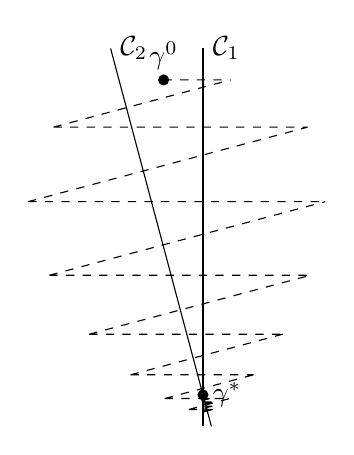
\begin{tikzpicture}
\fill (-0.500000,4.000000) circle (2pt) node[above] (gamma0) {$\gamma^0$};
\fill (0,0) circle (2pt) node[right] {$\gamma^*$};
\draw[dashed] (-0.500000,4.000000) -- (0.350000,4.000000)
(-1.898444,3.400415) -- (0.350000,4.000000)
(-1.898444,3.400415) -- (1.328911,3.400415)
(-2.219432,2.454190) -- (1.328911,3.400415)
(-2.219432,2.454190) -- (1.553603,2.454190)
(-1.950880,1.519661) -- (1.553603,2.454190)
(-1.950880,1.519661) -- (1.365616,1.519661)
(-1.444980,0.770169) -- (1.365616,1.519661)
(-1.444980,0.770169) -- (1.011486,0.770169)
(-0.919844,0.255148) -- (1.011486,0.770169)
(-0.919844,0.255148) -- (0.643891,0.255148)
(-0.486040,-0.046167) -- (0.643891,0.255148)
(-0.486040,-0.046167) -- (0.340228,-0.046167)
(-0.180221,-0.184954) -- (0.340228,-0.046167)
(-0.180221,-0.184954) -- (0.126154,-0.184954)
(0.004209,-0.217472) -- (0.126154,-0.184954)
(0.004209,-0.217472) -- (-0.002946,-0.217472)
(0.093772,-0.191681) -- (-0.002946,-0.217472)
(0.093772,-0.191681) -- (-0.065641,-0.191681)
(0.119666,-0.142266) -- (-0.065641,-0.191681)
(0.119666,-0.142266) -- (-0.083766,-0.142266)
(0.109394,-0.090756) -- (-0.083766,-0.142266)
(0.109394,-0.090756) -- (-0.076576,-0.090756)
(0.083372,-0.048103) -- (-0.076576,-0.090756)
(0.083372,-0.048103) -- (-0.058360,-0.048103)
(0.054625,-0.017974) -- (-0.058360,-0.048103)
(0.054625,-0.017974) -- (-0.038237,-0.017974)
(0.030058,0.000238) -- (-0.038237,-0.017974)
(0.030058,0.000238) -- (-0.021040,0.000238)
(0.012253,0.009116) -- (-0.021040,0.000238)
(0.012253,0.009116) -- (-0.008577,0.009116)
(0.001178,0.011717) -- (-0.008577,0.009116)
(0.001178,0.011717) -- (-0.000824,0.011717)
(-0.004475,0.010744) -- (-0.000824,0.011717)
(-0.004475,0.010744) -- (0.003133,0.010744)
(-0.006387,0.008205) -- (0.003133,0.010744)
(-0.006387,0.008205) -- (0.004471,0.008205)
(-0.006098,0.005387) -- (0.004471,0.008205)
(-0.006098,0.005387) -- (0.004268,0.005387)
(-0.004786,0.002973) -- (0.004268,0.005387)
(-0.004786,0.002973) -- (0.003350,0.002973)
(-0.003225,0.001219) -- (0.003350,0.002973)
(-0.003225,0.001219) -- (0.002258,0.001219)
(-0.001842,0.000126) -- (0.002258,0.001219)
(-0.001842,0.000126) -- (0.001289,0.000126)
(-0.000810,-0.000434) -- (0.001289,0.000126)
(-0.000810,-0.000434) -- (0.000567,-0.000434)
(-0.000149,-0.000625) -- (0.000567,-0.000434)
(-0.000149,-0.000625) -- (0.000105,-0.000625)
(0.000203,-0.000599) -- (0.000105,-0.000625)
(0.000203,-0.000599) -- (-0.000142,-0.000599)
(0.000337,-0.000471) -- (-0.000142,-0.000599)
(0.000337,-0.000471) -- (-0.000236,-0.000471)
(0.000338,-0.000318) -- (-0.000236,-0.000471)
(0.000338,-0.000318) -- (-0.000236,-0.000318)
(0.000273,-0.000182) -- (-0.000236,-0.000318)
(0.000273,-0.000182) -- (-0.000191,-0.000182)
(0.000189,-0.000080) -- (-0.000191,-0.000182)
(0.000189,-0.000080) -- (-0.000133,-0.000080)
(0.000112,-0.000015) -- (-0.000133,-0.000080)
(0.000112,-0.000015) -- (-0.000078,-0.000015)
(0.000052,0.000020) -- (-0.000078,-0.000015)
(0.000052,0.000020) -- (-0.000037,0.000020)
(0.000013,0.000033) -- (-0.000037,0.000020)
(0.000013,0.000033) -- (-0.000009,0.000033)
(-0.000008,0.000033) -- (-0.000009,0.000033)
(-0.000008,0.000033) -- (0.000006,0.000033)
(-0.000018,0.000027) -- (0.000006,0.000033)
(-0.000018,0.000027) -- (0.000012,0.000027)
(-0.000019,0.000019) -- (0.000012,0.000027)
(-0.000019,0.000019) -- (0.000013,0.000019)
(-0.000016,0.000011) -- (0.000013,0.000019)
(-0.000016,0.000011) -- (0.000011,0.000011)
(-0.000011,0.000005) -- (0.000011,0.000011)
(-0.000011,0.000005) -- (0.000008,0.000005)
(-0.000007,0.000001) -- (0.000008,0.000005)
(-0.000007,0.000001) -- (0.000005,0.000001)
(-0.000003,-0.000001) -- (0.000005,0.000001)
(-0.000003,-0.000001) -- (0.000002,-0.000001)
(-0.000001,-0.000002) -- (0.000002,-0.000001)
(-0.000001,-0.000002) -- (0.000001,-0.000002)
(0.000000,-0.000002) -- (0.000001,-0.000002)
(0.000000,-0.000002) -- (-0.000000,-0.000002)
(0.000001,-0.000002) -- (-0.000000,-0.000002)
(0.000001,-0.000002) -- (-0.000001,-0.000002)
(0.000001,-0.000001) -- (-0.000001,-0.000002)
(0.000001,-0.000001) -- (-0.000001,-0.000001)
(0.000001,-0.000001) -- (-0.000001,-0.000001)
(0.000001,-0.000001) -- (-0.000001,-0.000001)
(0.000001,-0.000000) -- (-0.000001,-0.000001)
(0.000001,-0.000000) -- (-0.000000,-0.000000)
(0.000000,-0.000000) -- (-0.000000,-0.000000)
(0.000000,-0.000000) -- (-0.000000,-0.000000)
(0.000000,0.000000) -- (-0.000000,-0.000000)
(0.000000,0.000000) -- (-0.000000,0.000000)
(0.000000,0.000000) -- (-0.000000,0.000000)
(0.000000,0.000000) -- (-0.000000,0.000000)
(-0.000000,0.000000) -- (-0.000000,0.000000)
(-0.000000,0.000000) -- (0.000000,0.000000)
(-0.000000,0.000000) -- (0.000000,0.000000)
(-0.000000,0.000000) -- (0.000000,0.000000)
(-0.000000,0.000000) -- (0.000000,0.000000)
(-0.000000,0.000000) -- (0.000000,0.000000)
(-0.000000,0.000000) -- (0.000000,0.000000)
(-0.000000,0.000000) -- (0.000000,0.000000)
(-0.000000,0.000000) -- (0.000000,0.000000)
(-0.000000,0.000000) -- (0.000000,0.000000)
(-0.000000,0.000000) -- (0.000000,0.000000)
(-0.000000,0.000000) -- (0.000000,0.000000)
(-0.000000,-0.000000) -- (0.000000,0.000000)
(-0.000000,-0.000000) -- (0.000000,-0.000000)
(-0.000000,-0.000000) -- (0.000000,-0.000000)
(-0.000000,-0.000000) -- (0.000000,-0.000000)
(-0.000000,-0.000000) -- (0.000000,-0.000000)
(-0.000000,-0.000000) -- (0.000000,-0.000000)
(0.000000,-0.000000) -- (0.000000,-0.000000)
(0.000000,-0.000000) -- (-0.000000,-0.000000)
(0.000000,-0.000000) -- (-0.000000,-0.000000)
(0.000000,-0.000000) -- (-0.000000,-0.000000)
(0.000000,-0.000000) -- (-0.000000,-0.000000)
(0.000000,-0.000000) -- (-0.000000,-0.000000)
(0.000000,-0.000000) -- (-0.000000,-0.000000)
(0.000000,-0.000000) -- (-0.000000,-0.000000)
(0.000000,-0.000000) -- (-0.000000,-0.000000)
(0.000000,-0.000000) -- (-0.000000,-0.000000)
(0.000000,-0.000000) -- (-0.000000,-0.000000)
(0.000000,-0.000000) -- (-0.000000,-0.000000)
(0.000000,0.000000) -- (-0.000000,-0.000000)
(0.000000,0.000000) -- (-0.000000,0.000000)
(0.000000,0.000000) -- (-0.000000,0.000000)
(0.000000,0.000000) -- (-0.000000,0.000000)
(-0.000000,0.000000) -- (-0.000000,0.000000)
(-0.000000,0.000000) -- (0.000000,0.000000)
(-0.000000,0.000000) -- (0.000000,0.000000)
(-0.000000,0.000000) -- (0.000000,0.000000)
(-0.000000,0.000000) -- (0.000000,0.000000)
(-0.000000,0.000000) -- (0.000000,0.000000)
(-0.000000,0.000000) -- (0.000000,0.000000)
(-0.000000,0.000000) -- (0.000000,0.000000)
(-0.000000,0.000000) -- (0.000000,0.000000)
(-0.000000,0.000000) -- (0.000000,0.000000)
(-0.000000,0.000000) -- (0.000000,0.000000)
(-0.000000,0.000000) -- (0.000000,0.000000)
(-0.000000,-0.000000) -- (0.000000,0.000000)
(-0.000000,-0.000000) -- (0.000000,-0.000000)
(-0.000000,-0.000000) -- (0.000000,-0.000000)
(-0.000000,-0.000000) -- (0.000000,-0.000000)
(0.000000,-0.000000) -- (0.000000,-0.000000)
(0.000000,-0.000000) -- (-0.000000,-0.000000)
(0.000000,-0.000000) -- (-0.000000,-0.000000)
(0.000000,-0.000000) -- (-0.000000,-0.000000)
(0.000000,-0.000000) -- (-0.000000,-0.000000)
(0.000000,-0.000000) -- (-0.000000,-0.000000)
(0.000000,-0.000000) -- (-0.000000,-0.000000)
(0.000000,-0.000000) -- (-0.000000,-0.000000)
(0.000000,-0.000000) -- (-0.000000,-0.000000)
(0.000000,-0.000000) -- (-0.000000,-0.000000)
(0.000000,-0.000000) -- (-0.000000,-0.000000)
(0.000000,-0.000000) -- (-0.000000,-0.000000)
(0.000000,0.000000) -- (-0.000000,-0.000000)
(0.000000,0.000000) -- (-0.000000,0.000000)
(0.000000,0.000000) -- (-0.000000,0.000000)
(0.000000,0.000000) -- (-0.000000,0.000000)
(-0.000000,0.000000) -- (-0.000000,0.000000)
(-0.000000,0.000000) -- (0.000000,0.000000)
(-0.000000,0.000000) -- (0.000000,0.000000)
(-0.000000,0.000000) -- (0.000000,0.000000)
(-0.000000,0.000000) -- (0.000000,0.000000)
(-0.000000,0.000000) -- (0.000000,0.000000)
(-0.000000,0.000000) -- (0.000000,0.000000)
(-0.000000,0.000000) -- (0.000000,0.000000)
(-0.000000,0.000000) -- (0.000000,0.000000)
(-0.000000,0.000000) -- (0.000000,0.000000)
(-0.000000,0.000000) -- (0.000000,0.000000)
(-0.000000,0.000000) -- (0.000000,0.000000)
(-0.000000,-0.000000) -- (0.000000,0.000000)
(-0.000000,-0.000000) -- (0.000000,-0.000000)
(-0.000000,-0.000000) -- (0.000000,-0.000000)
(-0.000000,-0.000000) -- (0.000000,-0.000000)
(0.000000,-0.000000) -- (0.000000,-0.000000)
(0.000000,-0.000000) -- (-0.000000,-0.000000)
(0.000000,-0.000000) -- (-0.000000,-0.000000)
(0.000000,-0.000000) -- (-0.000000,-0.000000)
(0.000000,-0.000000) -- (-0.000000,-0.000000)
(0.000000,-0.000000) -- (-0.000000,-0.000000)
(0.000000,-0.000000) -- (-0.000000,-0.000000)
(0.000000,-0.000000) -- (-0.000000,-0.000000)
(0.000000,-0.000000) -- (-0.000000,-0.000000)
(0.000000,-0.000000) -- (-0.000000,-0.000000)
(0.000000,-0.000000) -- (-0.000000,-0.000000)
(0.000000,-0.000000) -- (-0.000000,-0.000000)
(0.000000,0.000000) -- (-0.000000,-0.000000)
(0.000000,0.000000) -- (-0.000000,0.000000)
(0.000000,0.000000) -- (-0.000000,0.000000)
(0.000000,0.000000) -- (-0.000000,0.000000)
(0.000000,0.000000) -- (-0.000000,0.000000)
(0.000000,0.000000) -- (-0.000000,0.000000)
(-0.000000,0.000000) -- (-0.000000,0.000000)
(-0.000000,0.000000) -- (0.000000,0.000000)
(-0.000000,0.000000) -- (0.000000,0.000000)
;
\draw (-0.000000,-0.400000) -- (0.000000,4.400000) node[right] {$\mathcal{C}_1$};
\draw (0.106667,-0.400000) -- (-1.173333,4.400000) node[right] {$\mathcal{C}_2$};
\end{tikzpicture}

                    \subcaption{}\label{fig:schema_c}
\end{minipage}%
\caption{\label{alternate_projections} The trajectory of $\gamma^l$ given by the SK algorithm is illustrated for decreasing values of $\epsilon$ in (a) and (b). Overrelaxed projection typically accelerate the convergence rate.}
\end{figure}

\iffalse
\begin{figure}[ht!]
\begin{center}
\begin{tabular}{ccc}
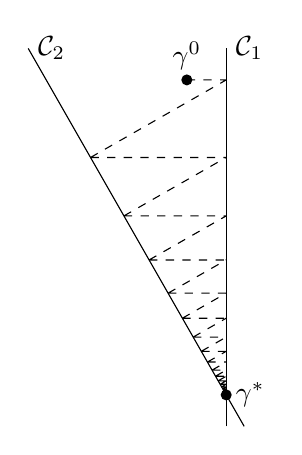
\begin{tikzpicture}
\fill (-0.500000,4.000000) circle (2pt) node[above] (gamma0) {$\gamma^0$};
\fill (0,0) circle (2pt) node[right] {$\gamma^*$};
\draw[dashed] (-0.500000,4.000000) -- (0.000000,4.000000)
(-1.723077,3.015385) -- (0.000000,4.000000)
(-1.723077,3.015385) -- (0.000000,3.015385)
(-1.298935,2.273136) -- (0.000000,3.015385)
(-1.298935,2.273136) -- (0.000000,2.273136)
(-0.979197,1.713595) -- (0.000000,2.273136)
(-0.979197,1.713595) -- (0.000000,1.713595)
(-0.738164,1.291787) -- (0.000000,1.713595)
(-0.738164,1.291787) -- (0.000000,1.291787)
(-0.556462,0.973809) -- (0.000000,1.291787)
(-0.556462,0.973809) -- (0.000000,0.973809)
(-0.419487,0.734102) -- (0.000000,0.973809)
(-0.419487,0.734102) -- (0.000000,0.734102)
(-0.316228,0.553400) -- (0.000000,0.734102)
(-0.316228,0.553400) -- (0.000000,0.553400)
(-0.238388,0.417178) -- (0.000000,0.553400)
(-0.238388,0.417178) -- (0.000000,0.417178)
(-0.179708,0.314488) -- (0.000000,0.417178)
(-0.179708,0.314488) -- (0.000000,0.314488)
(-0.135472,0.237076) -- (0.000000,0.314488)
(-0.135472,0.237076) -- (0.000000,0.237076)
(-0.102125,0.178719) -- (0.000000,0.237076)
(-0.102125,0.178719) -- (0.000000,0.178719)
(-0.076987,0.134726) -- (0.000000,0.178719)
(-0.076987,0.134726) -- (0.000000,0.134726)
(-0.058036,0.101563) -- (0.000000,0.134726)
(-0.058036,0.101563) -- (0.000000,0.101563)
(-0.043750,0.076563) -- (0.000000,0.101563)
(-0.043750,0.076563) -- (0.000000,0.076563)
(-0.032981,0.057717) -- (0.000000,0.076563)
(-0.032981,0.057717) -- (0.000000,0.057717)
(-0.024863,0.043509) -- (0.000000,0.057717)
(-0.024863,0.043509) -- (0.000000,0.043509)
(-0.018743,0.032799) -- (0.000000,0.043509)
(-0.018743,0.032799) -- (0.000000,0.032799)
(-0.014129,0.024726) -- (0.000000,0.032799)
(-0.014129,0.024726) -- (0.000000,0.024726)
(-0.010651,0.018639) -- (0.000000,0.024726)
(-0.010651,0.018639) -- (0.000000,0.018639)
(-0.008029,0.014051) -- (0.000000,0.018639)
(-0.008029,0.014051) -- (0.000000,0.014051)
(-0.006053,0.010592) -- (0.000000,0.014051)
(-0.006053,0.010592) -- (0.000000,0.010592)
(-0.004563,0.007985) -- (0.000000,0.010592)
(-0.004563,0.007985) -- (0.000000,0.007985)
(-0.003440,0.006020) -- (0.000000,0.007985)
(-0.003440,0.006020) -- (0.000000,0.006020)
(-0.002593,0.004538) -- (0.000000,0.006020)
(-0.002593,0.004538) -- (0.000000,0.004538)
(-0.001955,0.003421) -- (0.000000,0.004538)
(-0.001955,0.003421) -- (0.000000,0.003421)
(-0.001474,0.002579) -- (0.000000,0.003421)
(-0.001474,0.002579) -- (0.000000,0.002579)
(-0.001111,0.001944) -- (0.000000,0.002579)
(-0.001111,0.001944) -- (0.000000,0.001944)
(-0.000837,0.001465) -- (0.000000,0.001944)
(-0.000837,0.001465) -- (0.000000,0.001465)
(-0.000631,0.001105) -- (0.000000,0.001465)
(-0.000631,0.001105) -- (0.000000,0.001105)
(-0.000476,0.000833) -- (0.000000,0.001105)
(-0.000476,0.000833) -- (0.000000,0.000833)
(-0.000359,0.000628) -- (0.000000,0.000833)
(-0.000359,0.000628) -- (0.000000,0.000628)
(-0.000270,0.000473) -- (0.000000,0.000628)
(-0.000270,0.000473) -- (0.000000,0.000473)
(-0.000204,0.000357) -- (0.000000,0.000473)
(-0.000204,0.000357) -- (0.000000,0.000357)
(-0.000154,0.000269) -- (0.000000,0.000357)
(-0.000154,0.000269) -- (0.000000,0.000269)
(-0.000116,0.000203) -- (0.000000,0.000269)
(-0.000116,0.000203) -- (0.000000,0.000203)
(-0.000087,0.000153) -- (0.000000,0.000203)
(-0.000087,0.000153) -- (0.000000,0.000153)
(-0.000066,0.000115) -- (0.000000,0.000153)
(-0.000066,0.000115) -- (0.000000,0.000115)
(-0.000050,0.000087) -- (0.000000,0.000115)
(-0.000050,0.000087) -- (0.000000,0.000087)
(-0.000037,0.000065) -- (0.000000,0.000087)
(-0.000037,0.000065) -- (0.000000,0.000065)
(-0.000028,0.000049) -- (0.000000,0.000065)
(-0.000028,0.000049) -- (0.000000,0.000049)
(-0.000021,0.000037) -- (0.000000,0.000049)
(-0.000021,0.000037) -- (0.000000,0.000037)
(-0.000016,0.000028) -- (0.000000,0.000037)
(-0.000016,0.000028) -- (0.000000,0.000028)
(-0.000012,0.000021) -- (0.000000,0.000028)
(-0.000012,0.000021) -- (0.000000,0.000021)
(-0.000009,0.000016) -- (0.000000,0.000021)
(-0.000009,0.000016) -- (0.000000,0.000016)
(-0.000007,0.000012) -- (0.000000,0.000016)
(-0.000007,0.000012) -- (0.000000,0.000012)
(-0.000005,0.000009) -- (0.000000,0.000012)
(-0.000005,0.000009) -- (0.000000,0.000009)
(-0.000004,0.000007) -- (0.000000,0.000009)
(-0.000004,0.000007) -- (0.000000,0.000007)
(-0.000003,0.000005) -- (0.000000,0.000007)
(-0.000003,0.000005) -- (0.000000,0.000005)
(-0.000002,0.000004) -- (0.000000,0.000005)
(-0.000002,0.000004) -- (0.000000,0.000004)
(-0.000002,0.000003) -- (0.000000,0.000004)
(-0.000002,0.000003) -- (0.000000,0.000003)
(-0.000001,0.000002) -- (0.000000,0.000003)
(-0.000001,0.000002) -- (0.000000,0.000002)
(-0.000001,0.000002) -- (0.000000,0.000002)
(-0.000001,0.000002) -- (0.000000,0.000002)
(-0.000001,0.000001) -- (0.000000,0.000002)
(-0.000001,0.000001) -- (0.000000,0.000001)
(-0.000001,0.000001) -- (0.000000,0.000001)
(-0.000001,0.000001) -- (0.000000,0.000001)
(-0.000000,0.000001) -- (0.000000,0.000001)
(-0.000000,0.000001) -- (0.000000,0.000001)
(-0.000000,0.000001) -- (0.000000,0.000001)
(-0.000000,0.000001) -- (0.000000,0.000001)
(-0.000000,0.000000) -- (0.000000,0.000001)
(-0.000000,0.000000) -- (0.000000,0.000000)
(-0.000000,0.000000) -- (0.000000,0.000000)
(-0.000000,0.000000) -- (0.000000,0.000000)
(-0.000000,0.000000) -- (0.000000,0.000000)
(-0.000000,0.000000) -- (0.000000,0.000000)
(-0.000000,0.000000) -- (0.000000,0.000000)
(-0.000000,0.000000) -- (0.000000,0.000000)
(-0.000000,0.000000) -- (0.000000,0.000000)
(-0.000000,0.000000) -- (0.000000,0.000000)
(-0.000000,0.000000) -- (0.000000,0.000000)
(-0.000000,0.000000) -- (0.000000,0.000000)
(-0.000000,0.000000) -- (0.000000,0.000000)
(-0.000000,0.000000) -- (0.000000,0.000000)
(-0.000000,0.000000) -- (0.000000,0.000000)
(-0.000000,0.000000) -- (0.000000,0.000000)
(-0.000000,0.000000) -- (0.000000,0.000000)
(-0.000000,0.000000) -- (0.000000,0.000000)
(-0.000000,0.000000) -- (0.000000,0.000000)
(-0.000000,0.000000) -- (0.000000,0.000000)
(-0.000000,0.000000) -- (0.000000,0.000000)
(-0.000000,0.000000) -- (0.000000,0.000000)
(-0.000000,0.000000) -- (0.000000,0.000000)
(-0.000000,0.000000) -- (0.000000,0.000000)
(-0.000000,0.000000) -- (0.000000,0.000000)
(-0.000000,0.000000) -- (0.000000,0.000000)
(-0.000000,0.000000) -- (0.000000,0.000000)
(-0.000000,0.000000) -- (0.000000,0.000000)
(-0.000000,0.000000) -- (0.000000,0.000000)
(-0.000000,0.000000) -- (0.000000,0.000000)
(-0.000000,0.000000) -- (0.000000,0.000000)
(-0.000000,0.000000) -- (0.000000,0.000000)
(-0.000000,0.000000) -- (0.000000,0.000000)
(-0.000000,0.000000) -- (0.000000,0.000000)
(-0.000000,0.000000) -- (0.000000,0.000000)
(-0.000000,0.000000) -- (0.000000,0.000000)
(-0.000000,0.000000) -- (0.000000,0.000000)
(-0.000000,0.000000) -- (0.000000,0.000000)
(-0.000000,0.000000) -- (0.000000,0.000000)
(-0.000000,0.000000) -- (0.000000,0.000000)
(-0.000000,0.000000) -- (0.000000,0.000000)
(-0.000000,0.000000) -- (0.000000,0.000000)
(-0.000000,0.000000) -- (0.000000,0.000000)
(-0.000000,0.000000) -- (0.000000,0.000000)
(-0.000000,0.000000) -- (0.000000,0.000000)
(-0.000000,0.000000) -- (0.000000,0.000000)
(-0.000000,0.000000) -- (0.000000,0.000000)
(-0.000000,0.000000) -- (0.000000,0.000000)
(-0.000000,0.000000) -- (0.000000,0.000000)
(-0.000000,0.000000) -- (0.000000,0.000000)
(-0.000000,0.000000) -- (0.000000,0.000000)
(-0.000000,0.000000) -- (0.000000,0.000000)
(-0.000000,0.000000) -- (0.000000,0.000000)
(-0.000000,0.000000) -- (0.000000,0.000000)
(-0.000000,0.000000) -- (0.000000,0.000000)
(-0.000000,0.000000) -- (0.000000,0.000000)
(-0.000000,0.000000) -- (0.000000,0.000000)
(-0.000000,0.000000) -- (0.000000,0.000000)
(-0.000000,0.000000) -- (0.000000,0.000000)
(-0.000000,0.000000) -- (0.000000,0.000000)
(-0.000000,0.000000) -- (0.000000,0.000000)
(-0.000000,0.000000) -- (0.000000,0.000000)
(-0.000000,0.000000) -- (0.000000,0.000000)
(-0.000000,0.000000) -- (0.000000,0.000000)
(-0.000000,0.000000) -- (0.000000,0.000000)
(-0.000000,0.000000) -- (0.000000,0.000000)
(-0.000000,0.000000) -- (0.000000,0.000000)
(-0.000000,0.000000) -- (0.000000,0.000000)
(-0.000000,0.000000) -- (0.000000,0.000000)
(-0.000000,0.000000) -- (0.000000,0.000000)
(-0.000000,0.000000) -- (0.000000,0.000000)
(-0.000000,0.000000) -- (0.000000,0.000000)
(-0.000000,0.000000) -- (0.000000,0.000000)
(-0.000000,0.000000) -- (0.000000,0.000000)
(-0.000000,0.000000) -- (0.000000,0.000000)
(-0.000000,0.000000) -- (0.000000,0.000000)
(-0.000000,0.000000) -- (0.000000,0.000000)
(-0.000000,0.000000) -- (0.000000,0.000000)
(-0.000000,0.000000) -- (0.000000,0.000000)
(-0.000000,0.000000) -- (0.000000,0.000000)
(-0.000000,0.000000) -- (0.000000,0.000000)
(-0.000000,0.000000) -- (0.000000,0.000000)
(-0.000000,0.000000) -- (0.000000,0.000000)
(-0.000000,0.000000) -- (0.000000,0.000000)
(-0.000000,0.000000) -- (0.000000,0.000000)
(-0.000000,0.000000) -- (0.000000,0.000000)
(-0.000000,0.000000) -- (0.000000,0.000000)
;
\draw (-0.000000,-0.400000) -- (0.000000,4.400000) node[right] {$\mathcal{C}_1$};
\draw (0.228571,-0.400000) -- (-2.514286,4.400000) node[right] {$\mathcal{C}_2$};
\end{tikzpicture}
&
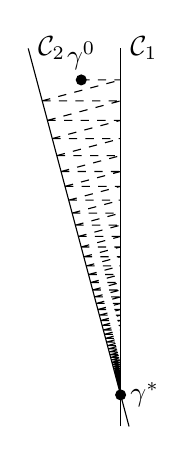
\begin{tikzpicture}
\fill (-0.500000,4.000000) circle (2pt) node[above] (gamma0) {$\gamma^0$};
\fill (0,0) circle (2pt) node[right] {$\gamma^*$};
\draw[dashed] (-0.500000,4.000000) -- (0.000000,4.000000)
(-0.995851,3.734440) -- (0.000000,4.000000)
(-0.995851,3.734440) -- (0.000000,3.734440)
(-0.929736,3.486510) -- (0.000000,3.734440)
(-0.929736,3.486510) -- (0.000000,3.486510)
(-0.868011,3.255041) -- (0.000000,3.486510)
(-0.868011,3.255041) -- (0.000000,3.255041)
(-0.810384,3.038938) -- (0.000000,3.255041)
(-0.810384,3.038938) -- (0.000000,3.038938)
(-0.756582,2.837183) -- (0.000000,3.038938)
(-0.756582,2.837183) -- (0.000000,2.837183)
(-0.706353,2.648822) -- (0.000000,2.837183)
(-0.706353,2.648822) -- (0.000000,2.648822)
(-0.659458,2.472967) -- (0.000000,2.648822)
(-0.659458,2.472967) -- (0.000000,2.472967)
(-0.615676,2.308787) -- (0.000000,2.472967)
(-0.615676,2.308787) -- (0.000000,2.308787)
(-0.574802,2.155506) -- (0.000000,2.308787)
(-0.574802,2.155506) -- (0.000000,2.155506)
(-0.536641,2.012402) -- (0.000000,2.155506)
(-0.536641,2.012402) -- (0.000000,2.012402)
(-0.501013,1.878799) -- (0.000000,2.012402)
(-0.501013,1.878799) -- (0.000000,1.878799)
(-0.467751,1.754065) -- (0.000000,1.878799)
(-0.467751,1.754065) -- (0.000000,1.754065)
(-0.436697,1.637613) -- (0.000000,1.754065)
(-0.436697,1.637613) -- (0.000000,1.637613)
(-0.407704,1.528891) -- (0.000000,1.637613)
(-0.407704,1.528891) -- (0.000000,1.528891)
(-0.380637,1.427388) -- (0.000000,1.528891)
(-0.380637,1.427388) -- (0.000000,1.427388)
(-0.355366,1.332624) -- (0.000000,1.427388)
(-0.355366,1.332624) -- (0.000000,1.332624)
(-0.331774,1.244151) -- (0.000000,1.332624)
(-0.331774,1.244151) -- (0.000000,1.244151)
(-0.309747,1.161552) -- (0.000000,1.244151)
(-0.309747,1.161552) -- (0.000000,1.161552)
(-0.289183,1.084436) -- (0.000000,1.161552)
(-0.289183,1.084436) -- (0.000000,1.084436)
(-0.269984,1.012440) -- (0.000000,1.084436)
(-0.269984,1.012440) -- (0.000000,1.012440)
(-0.252060,0.945225) -- (0.000000,1.012440)
(-0.252060,0.945225) -- (0.000000,0.945225)
(-0.235326,0.882471) -- (0.000000,0.945225)
(-0.235326,0.882471) -- (0.000000,0.882471)
(-0.219702,0.823884) -- (0.000000,0.882471)
(-0.219702,0.823884) -- (0.000000,0.823884)
(-0.205116,0.769186) -- (0.000000,0.823884)
(-0.205116,0.769186) -- (0.000000,0.769186)
(-0.191499,0.718120) -- (0.000000,0.769186)
(-0.191499,0.718120) -- (0.000000,0.718120)
(-0.178785,0.670444) -- (0.000000,0.718120)
(-0.178785,0.670444) -- (0.000000,0.670444)
(-0.166915,0.625933) -- (0.000000,0.670444)
(-0.166915,0.625933) -- (0.000000,0.625933)
(-0.155834,0.584377) -- (0.000000,0.625933)
(-0.155834,0.584377) -- (0.000000,0.584377)
(-0.145488,0.545580) -- (0.000000,0.584377)
(-0.145488,0.545580) -- (0.000000,0.545580)
(-0.135829,0.509359) -- (0.000000,0.545580)
(-0.135829,0.509359) -- (0.000000,0.509359)
(-0.126811,0.475543) -- (0.000000,0.509359)
(-0.126811,0.475543) -- (0.000000,0.475543)
(-0.118392,0.443972) -- (0.000000,0.475543)
(-0.118392,0.443972) -- (0.000000,0.443972)
(-0.110532,0.414496) -- (0.000000,0.443972)
(-0.110532,0.414496) -- (0.000000,0.414496)
(-0.103194,0.386978) -- (0.000000,0.414496)
(-0.103194,0.386978) -- (0.000000,0.386978)
(-0.096343,0.361286) -- (0.000000,0.386978)
(-0.096343,0.361286) -- (0.000000,0.361286)
(-0.089947,0.337301) -- (0.000000,0.361286)
(-0.089947,0.337301) -- (0.000000,0.337301)
(-0.083975,0.314907) -- (0.000000,0.337301)
(-0.083975,0.314907) -- (0.000000,0.314907)
(-0.078400,0.294000) -- (0.000000,0.314907)
(-0.078400,0.294000) -- (0.000000,0.294000)
(-0.073195,0.274482) -- (0.000000,0.294000)
(-0.073195,0.274482) -- (0.000000,0.274482)
(-0.068336,0.256259) -- (0.000000,0.274482)
(-0.068336,0.256259) -- (0.000000,0.256259)
(-0.063799,0.239246) -- (0.000000,0.256259)
(-0.063799,0.239246) -- (0.000000,0.239246)
(-0.059563,0.223362) -- (0.000000,0.239246)
(-0.059563,0.223362) -- (0.000000,0.223362)
(-0.055609,0.208533) -- (0.000000,0.223362)
(-0.055609,0.208533) -- (0.000000,0.208533)
(-0.051917,0.194689) -- (0.000000,0.208533)
(-0.051917,0.194689) -- (0.000000,0.194689)
(-0.048470,0.181763) -- (0.000000,0.194689)
(-0.048470,0.181763) -- (0.000000,0.181763)
(-0.045252,0.169696) -- (0.000000,0.181763)
(-0.045252,0.169696) -- (0.000000,0.169696)
(-0.042248,0.158430) -- (0.000000,0.169696)
(-0.042248,0.158430) -- (0.000000,0.158430)
(-0.039443,0.147912) -- (0.000000,0.158430)
(-0.039443,0.147912) -- (0.000000,0.147912)
(-0.036825,0.138092) -- (0.000000,0.147912)
(-0.036825,0.138092) -- (0.000000,0.138092)
(-0.034380,0.128924) -- (0.000000,0.138092)
(-0.034380,0.128924) -- (0.000000,0.128924)
(-0.032097,0.120365) -- (0.000000,0.128924)
(-0.032097,0.120365) -- (0.000000,0.120365)
(-0.029966,0.112374) -- (0.000000,0.120365)
(-0.029966,0.112374) -- (0.000000,0.112374)
(-0.027977,0.104913) -- (0.000000,0.112374)
(-0.027977,0.104913) -- (0.000000,0.104913)
(-0.026119,0.097948) -- (0.000000,0.104913)
(-0.026119,0.097948) -- (0.000000,0.097948)
(-0.024385,0.091445) -- (0.000000,0.097948)
(-0.024385,0.091445) -- (0.000000,0.091445)
(-0.022766,0.085374) -- (0.000000,0.091445)
(-0.022766,0.085374) -- (0.000000,0.085374)
(-0.021255,0.079706) -- (0.000000,0.085374)
(-0.021255,0.079706) -- (0.000000,0.079706)
(-0.019844,0.074415) -- (0.000000,0.079706)
(-0.019844,0.074415) -- (0.000000,0.074415)
(-0.018526,0.069474) -- (0.000000,0.074415)
(-0.018526,0.069474) -- (0.000000,0.069474)
(-0.017296,0.064862) -- (0.000000,0.069474)
(-0.017296,0.064862) -- (0.000000,0.064862)
(-0.016148,0.060556) -- (0.000000,0.064862)
(-0.016148,0.060556) -- (0.000000,0.060556)
(-0.015076,0.056535) -- (0.000000,0.060556)
(-0.015076,0.056535) -- (0.000000,0.056535)
(-0.014075,0.052782) -- (0.000000,0.056535)
(-0.014075,0.052782) -- (0.000000,0.052782)
(-0.013141,0.049278) -- (0.000000,0.052782)
(-0.013141,0.049278) -- (0.000000,0.049278)
(-0.012268,0.046006) -- (0.000000,0.049278)
(-0.012268,0.046006) -- (0.000000,0.046006)
(-0.011454,0.042952) -- (0.000000,0.046006)
(-0.011454,0.042952) -- (0.000000,0.042952)
(-0.010693,0.040100) -- (0.000000,0.042952)
(-0.010693,0.040100) -- (0.000000,0.040100)
(-0.009983,0.037438) -- (0.000000,0.040100)
(-0.009983,0.037438) -- (0.000000,0.037438)
(-0.009321,0.034952) -- (0.000000,0.037438)
(-0.009321,0.034952) -- (0.000000,0.034952)
(-0.008702,0.032632) -- (0.000000,0.034952)
(-0.008702,0.032632) -- (0.000000,0.032632)
(-0.008124,0.030466) -- (0.000000,0.032632)
(-0.008124,0.030466) -- (0.000000,0.030466)
(-0.007585,0.028443) -- (0.000000,0.030466)
(-0.007585,0.028443) -- (0.000000,0.028443)
(-0.007081,0.026555) -- (0.000000,0.028443)
(-0.007081,0.026555) -- (0.000000,0.026555)
(-0.006611,0.024792) -- (0.000000,0.026555)
(-0.006611,0.024792) -- (0.000000,0.024792)
(-0.006172,0.023146) -- (0.000000,0.024792)
(-0.006172,0.023146) -- (0.000000,0.023146)
(-0.005762,0.021609) -- (0.000000,0.023146)
(-0.005762,0.021609) -- (0.000000,0.021609)
(-0.005380,0.020174) -- (0.000000,0.021609)
(-0.005380,0.020174) -- (0.000000,0.020174)
(-0.005023,0.018835) -- (0.000000,0.020174)
(-0.005023,0.018835) -- (0.000000,0.018835)
(-0.004689,0.017585) -- (0.000000,0.018835)
(-0.004689,0.017585) -- (0.000000,0.017585)
(-0.004378,0.016417) -- (0.000000,0.017585)
(-0.004378,0.016417) -- (0.000000,0.016417)
(-0.004087,0.015327) -- (0.000000,0.016417)
(-0.004087,0.015327) -- (0.000000,0.015327)
(-0.003816,0.014310) -- (0.000000,0.015327)
(-0.003816,0.014310) -- (0.000000,0.014310)
(-0.003563,0.013360) -- (0.000000,0.014310)
(-0.003563,0.013360) -- (0.000000,0.013360)
(-0.003326,0.012473) -- (0.000000,0.013360)
(-0.003326,0.012473) -- (0.000000,0.012473)
(-0.003105,0.011645) -- (0.000000,0.012473)
(-0.003105,0.011645) -- (0.000000,0.011645)
(-0.002899,0.010872) -- (0.000000,0.011645)
(-0.002899,0.010872) -- (0.000000,0.010872)
(-0.002707,0.010150) -- (0.000000,0.010872)
(-0.002707,0.010150) -- (0.000000,0.010150)
(-0.002527,0.009476) -- (0.000000,0.010150)
(-0.002527,0.009476) -- (0.000000,0.009476)
(-0.002359,0.008847) -- (0.000000,0.009476)
(-0.002359,0.008847) -- (0.000000,0.008847)
(-0.002203,0.008259) -- (0.000000,0.008847)
(-0.002203,0.008259) -- (0.000000,0.008259)
(-0.002056,0.007711) -- (0.000000,0.008259)
(-0.002056,0.007711) -- (0.000000,0.007711)
(-0.001920,0.007199) -- (0.000000,0.007711)
(-0.001920,0.007199) -- (0.000000,0.007199)
(-0.001792,0.006721) -- (0.000000,0.007199)
(-0.001792,0.006721) -- (0.000000,0.006721)
(-0.001673,0.006275) -- (0.000000,0.006721)
(-0.001673,0.006275) -- (0.000000,0.006275)
(-0.001562,0.005858) -- (0.000000,0.006275)
(-0.001562,0.005858) -- (0.000000,0.005858)
(-0.001459,0.005469) -- (0.000000,0.005858)
(-0.001459,0.005469) -- (0.000000,0.005469)
(-0.001362,0.005106) -- (0.000000,0.005469)
(-0.001362,0.005106) -- (0.000000,0.005106)
(-0.001271,0.004767) -- (0.000000,0.005106)
(-0.001271,0.004767) -- (0.000000,0.004767)
(-0.001187,0.004451) -- (0.000000,0.004767)
(-0.001187,0.004451) -- (0.000000,0.004451)
(-0.001108,0.004155) -- (0.000000,0.004451)
;
\draw (-0.000000,-0.400000) -- (0.000000,4.400000) node[right] {$\mathcal{C}_1$};
\draw (0.106667,-0.400000) -- (-1.173333,4.400000) node[right] {$\mathcal{C}_2$};
\end{tikzpicture}
&
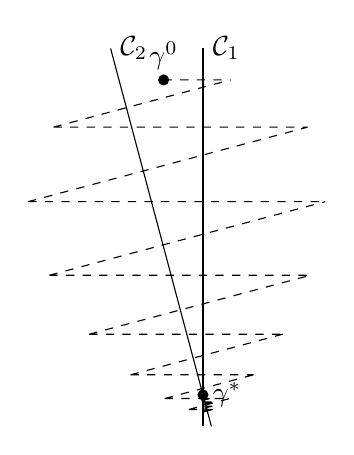
\begin{tikzpicture}
\fill (-0.500000,4.000000) circle (2pt) node[above] (gamma0) {$\gamma^0$};
\fill (0,0) circle (2pt) node[right] {$\gamma^*$};
\draw[dashed] (-0.500000,4.000000) -- (0.350000,4.000000)
(-1.898444,3.400415) -- (0.350000,4.000000)
(-1.898444,3.400415) -- (1.328911,3.400415)
(-2.219432,2.454190) -- (1.328911,3.400415)
(-2.219432,2.454190) -- (1.553603,2.454190)
(-1.950880,1.519661) -- (1.553603,2.454190)
(-1.950880,1.519661) -- (1.365616,1.519661)
(-1.444980,0.770169) -- (1.365616,1.519661)
(-1.444980,0.770169) -- (1.011486,0.770169)
(-0.919844,0.255148) -- (1.011486,0.770169)
(-0.919844,0.255148) -- (0.643891,0.255148)
(-0.486040,-0.046167) -- (0.643891,0.255148)
(-0.486040,-0.046167) -- (0.340228,-0.046167)
(-0.180221,-0.184954) -- (0.340228,-0.046167)
(-0.180221,-0.184954) -- (0.126154,-0.184954)
(0.004209,-0.217472) -- (0.126154,-0.184954)
(0.004209,-0.217472) -- (-0.002946,-0.217472)
(0.093772,-0.191681) -- (-0.002946,-0.217472)
(0.093772,-0.191681) -- (-0.065641,-0.191681)
(0.119666,-0.142266) -- (-0.065641,-0.191681)
(0.119666,-0.142266) -- (-0.083766,-0.142266)
(0.109394,-0.090756) -- (-0.083766,-0.142266)
(0.109394,-0.090756) -- (-0.076576,-0.090756)
(0.083372,-0.048103) -- (-0.076576,-0.090756)
(0.083372,-0.048103) -- (-0.058360,-0.048103)
(0.054625,-0.017974) -- (-0.058360,-0.048103)
(0.054625,-0.017974) -- (-0.038237,-0.017974)
(0.030058,0.000238) -- (-0.038237,-0.017974)
(0.030058,0.000238) -- (-0.021040,0.000238)
(0.012253,0.009116) -- (-0.021040,0.000238)
(0.012253,0.009116) -- (-0.008577,0.009116)
(0.001178,0.011717) -- (-0.008577,0.009116)
(0.001178,0.011717) -- (-0.000824,0.011717)
(-0.004475,0.010744) -- (-0.000824,0.011717)
(-0.004475,0.010744) -- (0.003133,0.010744)
(-0.006387,0.008205) -- (0.003133,0.010744)
(-0.006387,0.008205) -- (0.004471,0.008205)
(-0.006098,0.005387) -- (0.004471,0.008205)
(-0.006098,0.005387) -- (0.004268,0.005387)
(-0.004786,0.002973) -- (0.004268,0.005387)
(-0.004786,0.002973) -- (0.003350,0.002973)
(-0.003225,0.001219) -- (0.003350,0.002973)
(-0.003225,0.001219) -- (0.002258,0.001219)
(-0.001842,0.000126) -- (0.002258,0.001219)
(-0.001842,0.000126) -- (0.001289,0.000126)
(-0.000810,-0.000434) -- (0.001289,0.000126)
(-0.000810,-0.000434) -- (0.000567,-0.000434)
(-0.000149,-0.000625) -- (0.000567,-0.000434)
(-0.000149,-0.000625) -- (0.000105,-0.000625)
(0.000203,-0.000599) -- (0.000105,-0.000625)
(0.000203,-0.000599) -- (-0.000142,-0.000599)
(0.000337,-0.000471) -- (-0.000142,-0.000599)
(0.000337,-0.000471) -- (-0.000236,-0.000471)
(0.000338,-0.000318) -- (-0.000236,-0.000471)
(0.000338,-0.000318) -- (-0.000236,-0.000318)
(0.000273,-0.000182) -- (-0.000236,-0.000318)
(0.000273,-0.000182) -- (-0.000191,-0.000182)
(0.000189,-0.000080) -- (-0.000191,-0.000182)
(0.000189,-0.000080) -- (-0.000133,-0.000080)
(0.000112,-0.000015) -- (-0.000133,-0.000080)
(0.000112,-0.000015) -- (-0.000078,-0.000015)
(0.000052,0.000020) -- (-0.000078,-0.000015)
(0.000052,0.000020) -- (-0.000037,0.000020)
(0.000013,0.000033) -- (-0.000037,0.000020)
(0.000013,0.000033) -- (-0.000009,0.000033)
(-0.000008,0.000033) -- (-0.000009,0.000033)
(-0.000008,0.000033) -- (0.000006,0.000033)
(-0.000018,0.000027) -- (0.000006,0.000033)
(-0.000018,0.000027) -- (0.000012,0.000027)
(-0.000019,0.000019) -- (0.000012,0.000027)
(-0.000019,0.000019) -- (0.000013,0.000019)
(-0.000016,0.000011) -- (0.000013,0.000019)
(-0.000016,0.000011) -- (0.000011,0.000011)
(-0.000011,0.000005) -- (0.000011,0.000011)
(-0.000011,0.000005) -- (0.000008,0.000005)
(-0.000007,0.000001) -- (0.000008,0.000005)
(-0.000007,0.000001) -- (0.000005,0.000001)
(-0.000003,-0.000001) -- (0.000005,0.000001)
(-0.000003,-0.000001) -- (0.000002,-0.000001)
(-0.000001,-0.000002) -- (0.000002,-0.000001)
(-0.000001,-0.000002) -- (0.000001,-0.000002)
(0.000000,-0.000002) -- (0.000001,-0.000002)
(0.000000,-0.000002) -- (-0.000000,-0.000002)
(0.000001,-0.000002) -- (-0.000000,-0.000002)
(0.000001,-0.000002) -- (-0.000001,-0.000002)
(0.000001,-0.000001) -- (-0.000001,-0.000002)
(0.000001,-0.000001) -- (-0.000001,-0.000001)
(0.000001,-0.000001) -- (-0.000001,-0.000001)
(0.000001,-0.000001) -- (-0.000001,-0.000001)
(0.000001,-0.000000) -- (-0.000001,-0.000001)
(0.000001,-0.000000) -- (-0.000000,-0.000000)
(0.000000,-0.000000) -- (-0.000000,-0.000000)
(0.000000,-0.000000) -- (-0.000000,-0.000000)
(0.000000,0.000000) -- (-0.000000,-0.000000)
(0.000000,0.000000) -- (-0.000000,0.000000)
(0.000000,0.000000) -- (-0.000000,0.000000)
(0.000000,0.000000) -- (-0.000000,0.000000)
(-0.000000,0.000000) -- (-0.000000,0.000000)
(-0.000000,0.000000) -- (0.000000,0.000000)
(-0.000000,0.000000) -- (0.000000,0.000000)
(-0.000000,0.000000) -- (0.000000,0.000000)
(-0.000000,0.000000) -- (0.000000,0.000000)
(-0.000000,0.000000) -- (0.000000,0.000000)
(-0.000000,0.000000) -- (0.000000,0.000000)
(-0.000000,0.000000) -- (0.000000,0.000000)
(-0.000000,0.000000) -- (0.000000,0.000000)
(-0.000000,0.000000) -- (0.000000,0.000000)
(-0.000000,0.000000) -- (0.000000,0.000000)
(-0.000000,0.000000) -- (0.000000,0.000000)
(-0.000000,-0.000000) -- (0.000000,0.000000)
(-0.000000,-0.000000) -- (0.000000,-0.000000)
(-0.000000,-0.000000) -- (0.000000,-0.000000)
(-0.000000,-0.000000) -- (0.000000,-0.000000)
(-0.000000,-0.000000) -- (0.000000,-0.000000)
(-0.000000,-0.000000) -- (0.000000,-0.000000)
(0.000000,-0.000000) -- (0.000000,-0.000000)
(0.000000,-0.000000) -- (-0.000000,-0.000000)
(0.000000,-0.000000) -- (-0.000000,-0.000000)
(0.000000,-0.000000) -- (-0.000000,-0.000000)
(0.000000,-0.000000) -- (-0.000000,-0.000000)
(0.000000,-0.000000) -- (-0.000000,-0.000000)
(0.000000,-0.000000) -- (-0.000000,-0.000000)
(0.000000,-0.000000) -- (-0.000000,-0.000000)
(0.000000,-0.000000) -- (-0.000000,-0.000000)
(0.000000,-0.000000) -- (-0.000000,-0.000000)
(0.000000,-0.000000) -- (-0.000000,-0.000000)
(0.000000,-0.000000) -- (-0.000000,-0.000000)
(0.000000,0.000000) -- (-0.000000,-0.000000)
(0.000000,0.000000) -- (-0.000000,0.000000)
(0.000000,0.000000) -- (-0.000000,0.000000)
(0.000000,0.000000) -- (-0.000000,0.000000)
(-0.000000,0.000000) -- (-0.000000,0.000000)
(-0.000000,0.000000) -- (0.000000,0.000000)
(-0.000000,0.000000) -- (0.000000,0.000000)
(-0.000000,0.000000) -- (0.000000,0.000000)
(-0.000000,0.000000) -- (0.000000,0.000000)
(-0.000000,0.000000) -- (0.000000,0.000000)
(-0.000000,0.000000) -- (0.000000,0.000000)
(-0.000000,0.000000) -- (0.000000,0.000000)
(-0.000000,0.000000) -- (0.000000,0.000000)
(-0.000000,0.000000) -- (0.000000,0.000000)
(-0.000000,0.000000) -- (0.000000,0.000000)
(-0.000000,0.000000) -- (0.000000,0.000000)
(-0.000000,-0.000000) -- (0.000000,0.000000)
(-0.000000,-0.000000) -- (0.000000,-0.000000)
(-0.000000,-0.000000) -- (0.000000,-0.000000)
(-0.000000,-0.000000) -- (0.000000,-0.000000)
(0.000000,-0.000000) -- (0.000000,-0.000000)
(0.000000,-0.000000) -- (-0.000000,-0.000000)
(0.000000,-0.000000) -- (-0.000000,-0.000000)
(0.000000,-0.000000) -- (-0.000000,-0.000000)
(0.000000,-0.000000) -- (-0.000000,-0.000000)
(0.000000,-0.000000) -- (-0.000000,-0.000000)
(0.000000,-0.000000) -- (-0.000000,-0.000000)
(0.000000,-0.000000) -- (-0.000000,-0.000000)
(0.000000,-0.000000) -- (-0.000000,-0.000000)
(0.000000,-0.000000) -- (-0.000000,-0.000000)
(0.000000,-0.000000) -- (-0.000000,-0.000000)
(0.000000,-0.000000) -- (-0.000000,-0.000000)
(0.000000,0.000000) -- (-0.000000,-0.000000)
(0.000000,0.000000) -- (-0.000000,0.000000)
(0.000000,0.000000) -- (-0.000000,0.000000)
(0.000000,0.000000) -- (-0.000000,0.000000)
(-0.000000,0.000000) -- (-0.000000,0.000000)
(-0.000000,0.000000) -- (0.000000,0.000000)
(-0.000000,0.000000) -- (0.000000,0.000000)
(-0.000000,0.000000) -- (0.000000,0.000000)
(-0.000000,0.000000) -- (0.000000,0.000000)
(-0.000000,0.000000) -- (0.000000,0.000000)
(-0.000000,0.000000) -- (0.000000,0.000000)
(-0.000000,0.000000) -- (0.000000,0.000000)
(-0.000000,0.000000) -- (0.000000,0.000000)
(-0.000000,0.000000) -- (0.000000,0.000000)
(-0.000000,0.000000) -- (0.000000,0.000000)
(-0.000000,0.000000) -- (0.000000,0.000000)
(-0.000000,-0.000000) -- (0.000000,0.000000)
(-0.000000,-0.000000) -- (0.000000,-0.000000)
(-0.000000,-0.000000) -- (0.000000,-0.000000)
(-0.000000,-0.000000) -- (0.000000,-0.000000)
(0.000000,-0.000000) -- (0.000000,-0.000000)
(0.000000,-0.000000) -- (-0.000000,-0.000000)
(0.000000,-0.000000) -- (-0.000000,-0.000000)
(0.000000,-0.000000) -- (-0.000000,-0.000000)
(0.000000,-0.000000) -- (-0.000000,-0.000000)
(0.000000,-0.000000) -- (-0.000000,-0.000000)
(0.000000,-0.000000) -- (-0.000000,-0.000000)
(0.000000,-0.000000) -- (-0.000000,-0.000000)
(0.000000,-0.000000) -- (-0.000000,-0.000000)
(0.000000,-0.000000) -- (-0.000000,-0.000000)
(0.000000,-0.000000) -- (-0.000000,-0.000000)
(0.000000,-0.000000) -- (-0.000000,-0.000000)
(0.000000,0.000000) -- (-0.000000,-0.000000)
(0.000000,0.000000) -- (-0.000000,0.000000)
(0.000000,0.000000) -- (-0.000000,0.000000)
(0.000000,0.000000) -- (-0.000000,0.000000)
(0.000000,0.000000) -- (-0.000000,0.000000)
(0.000000,0.000000) -- (-0.000000,0.000000)
(-0.000000,0.000000) -- (-0.000000,0.000000)
(-0.000000,0.000000) -- (0.000000,0.000000)
(-0.000000,0.000000) -- (0.000000,0.000000)
;
\draw (-0.000000,-0.400000) -- (0.000000,4.400000) node[right] {$\mathcal{C}_1$};
\draw (0.106667,-0.400000) -- (-1.173333,4.400000) node[right] {$\mathcal{C}_2$};
\end{tikzpicture}
\\
(a)&(b)&(c)
\end{tabular}
\caption{\label{alternate_projections} The trajectory of $\gamma^l$ given by the SK algorithm is illustrated for decreasing values of $\epsilon$ in (a) and (b). In order to accelerate the convergence rate, over-relaxed projections are here considered (c).}
\end{center}
\end{figure}
\fi


\subsection{Overrelaxed projections}

We define the $\omega$-overrelaxed projection operator $P^\omega_{\Ccal_k}$ as
\begin{equation}\label{eq:def_or_proj}
\log P^\omega_{\Ccal_k}(\gamma) = (1-\omega) \log \gamma + \omega \log P_{\Ccal_k}(\gamma),
\end{equation}
where the logarithm is taken coordinate-wise. Note that $P_{\Ccal_k}^0$ is the identity, $P_{\Ccal_k}^1 = P_{\Ccal_k}$ is the standard Bregman projection and $P_{\Ccal_k}^2$ is an involution (in particular because $\Ccal_k$ is an affine subspace). A naive algorithm would then consist in iteratively applying $P^\omega_{\Ccal_2}\circ P^\omega_{\Ccal_1}$ for some choice of $\omega$. This algorithm, while it may behave well in practice, has no convergence guarantee---it sometimes does not convergence even for reasonable values of $\omega$. Our goal in this section is to modify this algorithm to make it robust and garantee convergence.

Duality gives another point of view on the iterative overrelaxed Bregman projections. They indeed correspond to a successive overelaxation (SOR) algorithm on the dual objective $E$. This can be seen by using the relationships gievn after equation~\eqref{DROT}:
\begin{align}\label{SORdual}
\alpha^{\ell+1} &= (1-\omega)\alpha^{\ell} + \omega \arg \max_\alpha E(\alpha,\beta^{\ell})\\
\beta^{\ell + 1}&=(1-\omega) \beta^{\ell} + \omega \arg \max_\beta E(\alpha^{\ell+1},\beta).
\end{align} 

{\color{blue} \begin{proposition} 
State here that the fixed points of   $\gamma^{l+1} =P^\theta_{\Ccal_2}(P^\theta_{\Ccal_1}(\gamma^l))$ are the same than $\gamma^{l+1} =P_{\Ccal_2}(P_{\Ccal_1}(\gamma^l))$? lenaic: what is exactly needed? I can think of it tomorow.
\end{proposition}}
\subsection{Lyapunov function}
Convergence of the successive overrelaxed projection cannot be guaranteed in general. In order to derive a robust algorithm with provable convergence, we introduce the Lyapunov function 
\begin{equation}\label{eq:lyapunov_function}
F(\gamma) = \KL(\gamma^*, \gamma),
\end{equation}
where $\gamma^*$ denotes the solution of the regularized OT problem. We will use this function to enforce the strict descent criterion $F(\gamma^{k+1}) < F(\gamma^k)$ as long as the process has not converged.
%
The choice of \eqref{eq:lyapunov_function} as a Lyapunov function is of course related to the fact that Bregman projections are used throughout the algorithm. Further, we will show (Lemma \ref{lemma:lyapunov_decrease}) that its decrease is very easy to compute and this descent criterion still allows enough freedom in the choice of the overrelaxation parameter.

Crucial properties of this Lyapunov function are gathered in the next lemma.
\begin{lemma} \label{lemma:lyapunov_decrease}
	For any $M \in \IR_+^*$, the sublevel set $\left\{ \gamma \mid F(\gamma) \le M \right\}$ is compact.
%\end{lemma}
%\begin{lemma}
	Moreover, for $\gamma$ in $\IR^{mn}_{+*}$, the decrease of the Lyapunov function after an overrelaxed projection can be computed as
	\begin{equation} \label{eq:kl_diff_scal}
	F(\gamma) - F(P^\omega_{\Ccal_k}(\gamma)) = 
	\scal{\mu^k}{\varphi_\omega \left((A_k \gamma) \oslash \mu^k \right)},
	\end{equation}
	where
	\begin{equation}
	\varphi_\omega(x) = x(1-x^{-\omega}) - \omega \log x
	\end{equation}
	is a real function, applied coordinate-wise.
\end{lemma}

\begin{proof}
The fact that the Kullback-Leibler divergence is jointly lower semicontinuous implies in particular that $K$ is closed. Moreover, $K\subset \mathbb{R}^{n_1\times n_2}_+$ is bounded because $F$ is the sum of nonnegative, coercive functions of each component of its argument $\gamma$.
%\end{proof}
%\begin{proof}
%
Formula \eqref{eq:kl_diff_scal} comes the expression $F(\gamma^1)-F(\gamma^2)= \sum_{i,j}\left(\gamma^*_{i,j}\log(\gamma^2_{i,j}/\gamma^1_{i,j})+\gamma^1_{i,j}-\gamma^2_{i,j}\right)$ and the relations \eqref{eq:def_or_proj} and \eqref{scaling}.
\end{proof}

\iffalse
\begin{proof}
	First note that K is closed in $\IR_{+*}^{n_1 n_2}$, by continuity of $F$.
	For $\gamma \in K$, one has:
	\begin{align*}
	F(\gamma) &= \scal{\gamma^*}{\log \gamma^* - 1} + \scal{\gamma}{1} - \scal{\gamma^*}{\log \gamma}\\
	\sum_{i,j} \gamma_{i,j} - \gamma^*_{i,j} \log \gamma_{i,j} &\le M - \scal{\gamma^*}{\log \gamma^* - 1} .
	\end{align*}
	By concavity, the logarithm admits a simple upper bound: $\log \gamma_{i,j} \le \frac{\gamma_{i,j}}{e}$. Moreover, since $\gamma^*$ is a solution of the problem, each of its coordinates is at most 1.
	\begin{align*}
	\sum_{i,j} \gamma_{i,j} &\le \frac{M - \scal{\gamma^*}{\log \gamma^*-1}}{1-\frac{1}{e}} =: M'.
	\end{align*}
	Therefore each coordinate $\gamma_{i,j}$ is bounded above by $M'$.
	
	Let us show that the coordinates are bounded below by a strictly positive number; from which it can be deduced that $K$ is bounded and closed in $\IR^{n_1 n_2}$, and therefore compact.
	\begin{align*}
	F(\gamma)
	&\ge \scal{\gamma^*}{\log \gamma^*} - \sum_{i,j} \gamma^*_{i,j} \log(\gamma_{i,j}) - 1\\
	&\ge \scal{\gamma^*}{\log \gamma^*} - \gamma^*_{i_0,j_0} \log(\gamma_{i_0,j_0}) - 1 - \log M',
	\end{align*}
	where the last equation derives from $\log(y_{i,j}) \le \log M'$, and $\sum_{(i,j)\neq(i_0,j_0)} \gamma^*_{i,j} \le 1$.
	Finally:
	\[
	\log(\gamma_{i_0,j_0}) \ge \frac{\scal{\gamma^*}{\log \gamma^*} - M - \log M' - 1}{\gamma^*_{i_0,j_0}},
	\]
	and $K$ is thus compact.
\end{proof}
\fi

%Note that the difference $F(\gamma) - F(P^\omega_{\Ccal_k}(\gamma))$ may be calculated without knowing $\gamma^*$, as shown by the following lemma.

It follows from Lemma \ref{lemma:lyapunov_decrease} that the decrease of $F$ for an overrelaxed projection is very cheap to estimate, since its computational cost is linear with respect to the dimension of data $\mu^k$. In Figure \ref{phi_omega}, we display the function  $\varphi_\omega(x)$. Notice that for the SK algorithm, which corresponds to $\omega=1$, the function $\varphi_\omega$ is always nonnegative. For other values $1\le\omega<2$, it is nonnegative for $x$ close to 1.

\begin{figure}[ht!]
\begin{center}
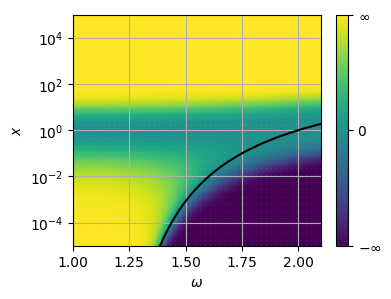
\includegraphics[width=7cm]{images/cvgce_zone}
\caption{\label{phi_omega} Value of $\varphi_\omega(x)$. The function is positive above the black line, negative below. For any relaxation parameter $\omega$ smaller than $2$, there exists a neighborhood of $1$ on which $\varphi_\omega(\cdot)$ is positive.}
%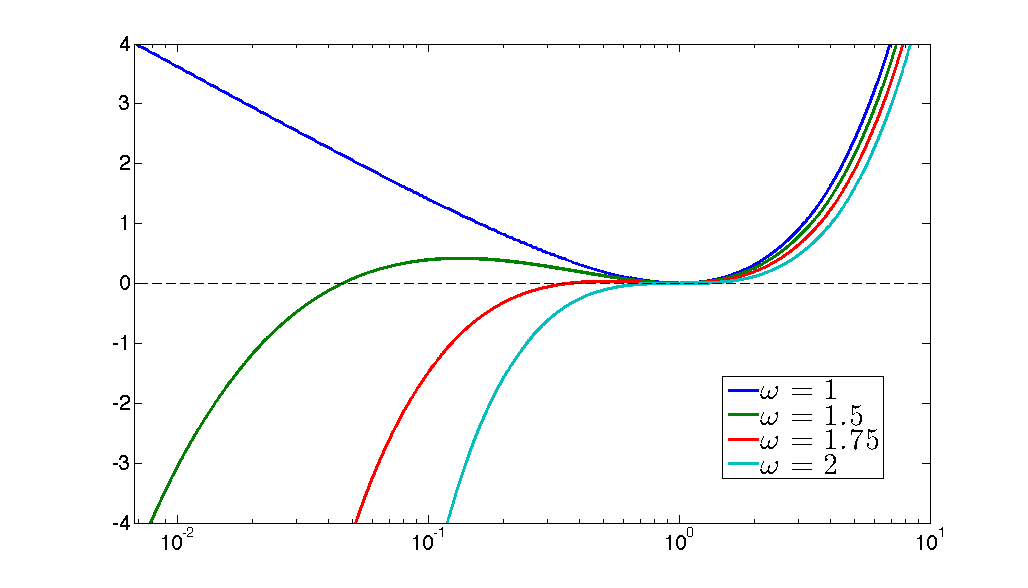
\includegraphics[width=11cm]{phi_omega.png}
%\caption{\label{phi_omega} Plot of functions $\varphi_\omega(x)$ for different values $1\leq \omega\leq 2$ and   $x\in[10^{-2}, 10^1]$.}
\end{center}
\end{figure}

\subsection{Proposed algorithm}
We first give a general convergence result that later serves as a basis to design an explicit algorithm.
\begin{theorem}\label{thm:algo}
Let $\theta_1$ and $\theta_2$ be two continuous functions of $\gamma$ such that
	\begin{equation}\label{eq:cond_theta_k}
	\forall \gamma \in \IR_{+*}^{n_1 n_2},\quad
	F(P_{\Ccal_k}^{\theta_k(\gamma)}(\gamma)) \le F(\gamma) ,
	\end{equation}
	where the inequality is strict whenever $\gamma \notin \Ccal_k$.
	Consider the sequence defined by $\gamma^0 = e^{-c/\epsilon}$ and
	\begin{align*}
	\tilde{\gamma}^{l+1} &= P_{\Ccal_1}^{\theta_1(\gamma^l)}(\gamma^l) \\
	\gamma^{l+1} &= P_{\Ccal_2}^{\theta_2(\tilde{\gamma}^{l+1})}(\tilde{\gamma}^{l+1}).
	\end{align*}
	Then the sequence $(\gamma^l)$ converges to $\gamma^*$.
\end{theorem}


\begin{lemma}[\cite{cuturi13}]
	\label{lemma:trivial_intersection}
	Let us take $\gamma^0$ in $\IR_{+*}^{n_1 n_2}$,
	and denote
	\[
	S = \left\{
	\diag(a) \gamma^0 \diag(b),\quad
	(a,b) \in \IR_{+*}^{n_1 + n_2}
	\right\}
	\]
	the set of matrices that are diagonally similar to $\gamma^0$.
	Then the set $S \cap \Ccal_1 \cap \Ccal_2$ contains exactly one element $\gamma^* = P_{\Ccal_1 \cap \Ccal_2}(\gamma^0)$.
\end{lemma}


\begin{proof}[Proof of the theorem]
	First of all, notice that the operators $P_{\Ccal_k}^\theta$ apply a scaling to lines or columns of matrices. All $(\gamma^l)$ are thus diagonally similar to $\gamma^0$:
	\[
	\forall l\ge0,\quad \gamma^l \in S
	\]
	By construction of the functions $\theta_k$, the sequence of values of the Lyapunov function $(F(\gamma^l))$ is non-increasing. Hence $(\gamma^l)$ is precompact.
	%
	If $\xi$ is a cluster point of $(\gamma^l)$, let us define
	\begin{align*}
	\tilde{\xi} &= P_{\Ccal_1}^{\theta_1(\xi)}(\xi) \\
	\xi' &= P_{\Ccal_2}^{\theta_2(\tilde{\xi})}(\tilde{\xi}).
	\end{align*}
	Then by continuity of the applications, $F(\xi) = F(\tilde{\xi}) = F(\xi')$.
	From the hypothesis made on $\theta_1$ and $\theta_2$, it can be deduced that $\xi$ is in $\Ccal_1$ and that $\tilde{\xi}$ is in $\Ccal_2$. Therefore $\xi' = \tilde{\xi} = \xi$ is in the intersection $\Ccal_1 \cap \Ccal_2$.
	By Lemma \ref{lemma:trivial_intersection}, $\xi = \gamma^*$, and the whole sequence $(\gamma^l)$ converges to the solution.
\end{proof}



%{\color{red} 
%	TODO Construire les bonnes fonctions $\theta_k(\gamma)$.}

To construct explicitly functions $\theta_k$ as needed in Theorem~\ref{thm:algo}, we need the following lemma.
\begin{lemma}\label{lemma:F_P_theta}
	Let $1\le \theta < \omega$. Then, for any $\gamma \in \IR_{+*}^{nm}$, one has
	\begin{equation}\label{eq:F_P_theta}
	F(P^\theta_{\Ccal_k}(\gamma)) \le F(P^\omega_{\Ccal_k}(\gamma)).
	\end{equation}
	Moreover, equality occurs if and only if $\gamma \in \Ccal_k$.
\end{lemma}
\begin{proof}
	Thanks to lemma \ref{lemma:lyapunov_decrease}, one knows that
	\[
	F(P^\theta_{\Ccal_k}(\gamma)) - F(P^\omega_{\Ccal_k}(\gamma))
	= \scal{\mu^k}{(\varphi_\omega - \varphi_\theta) \left( \frac{A_k \gamma}{\mu^k} \right) } .
	\]
	Moreover, the function that maps $t \in [1,\infty)$ to $\varphi_t(x)$ is non-increasing:
	$\partial_t \varphi_t(x) =  (x^{1-t} - 1)\log x.$
	For $x\neq 1$, it is even strictly decreasing.
	Thus inequality \eqref{eq:F_P_theta} is valid, with equality \emph{iff} $A_k \gamma = \mu$.
\end{proof}

We now argue that a good choice for the functions $\theta_k$ may be constructed as follows. Pick a target parameter $\theta_0 \in [1;2)$ and a small security distance $\delta>0$. Define the functions $\Theta^*$ and $\Theta$ as
	\begin{align}
	\label{eq:Theta_opt}
	\Theta^*(u) &= \sup \left\{\omega \in [1;2]  \mid \varphi_\omega\left(\min u\right) \ge 0 \right\} ,\\
	\label{eq:Theta}
	\Theta(u) &= \min(\max(1,\Theta^*(u)-\delta),\theta_0),
	\end{align}
	where $\min u$ denotes the smallest coordinate of the vector $u$. 

\begin{proposition}\label{prop:thetachoice}
	The function
	\begin{equation}
	\label{eq:theta_k}
	\theta_k(\gamma) =\Theta\left ((A_k \gamma)\oslash \mu^k\right)
	\end{equation}
	is continuous and verifies the descent condition (\ref{eq:cond_theta_k}).
\end{proposition}
This construction has several advantages:
\begin{itemize}
\item it allows to choose arbitrarily the parameter $\theta_0$ that will be used eventually when the algorithm is close to convergence (we motivate what are good choices for $\theta_0$ in section \ref{section:local});
\item it is also an easy approach to having an adaptive method, as the approximation of $\Theta_k^*$ has a negligible cost (it only require to solve a one dimensional problem that depends on the smallest value of $(A_k \gamma)\oslash \mu^k$, which can be done in a few iterations of Newton's method).
\item experiments show that this is often an excellent choice in practice.
\end{itemize}

\begin{proof}
Looking at Figure~\ref{phi_omega} can help understanding this proof.	Since the partial derivative of $\partial_\omega \varphi_\omega(x)$ is nonzero for any $x<1$, the implicit function theorem proves the continuity of $\Theta^*$.
	The function $\Theta^*\left((A_k \gamma)\oslash \mu^k)\right)$ is such that every term in relation (\ref{eq:kl_diff_scal}) is non-negative.
	Therefore, by lemma \ref{lemma:F_P_theta}, using this parameter minus $\delta$ ensures the strong decrease (\ref{eq:cond_theta_k}) of the Lyapunov function.
	Constraining the parameter to $[1,\theta_0]$ preserves this properties.% as using $\theta=1$ always satisfies inequality \eqref{eq:cond_theta_k} and using $\theta=\theta_0$ when it is smaller than $\Theta^*\left(\frac{A_k \gamma}{\mu^k}\right)$ does as well.
\end{proof}

The resulting algorithm, which is proved to be convergent by Theorem~\ref{thm:algo}, is written in pseudo-code in Algorithm \ref{SOR}. It uses the function $\Theta$ defined implicitely in \eqref{eq:Theta}, which in practice is approximated with a few iterations of Newton's method on the function $\omega \mapsto \varphi_\omega(\min u)$ which decreasing is as can be seen on Figure~\ref{phi_omega}. Note that with the choice $\theta_0=1$, one recovers exactly the original SK algorithm.

\begin{algorithm}
\caption{Overrelaxed SK algorithm }
\label{SOR}
\begin{algorithmic}
\REQUIRE $\mu^1\in \IR^{n_1}$, $\mu^2\in \IR^{n_2}$, $c\in \IR^{n_1\times n_2}_+$
\STATE Set $a=\mathbf{1}_{n_1}$, $b=\mathbf{1}_{n_2}$, $\gamma^0=e^{-c/\epsilon}$, $\theta_0\in[1;2)$ and $\eta>0$
\WHILE {$||a\otimes \gamma^0b-  \mu_1||>\eta$}
\STATE $\tilde a=\mu_1\oslash (\gamma^0 b)$, 
\STATE $\omega=\Theta(a\oslash\tilde a)$
%\IF{ $\langle \mu^1,\varphi_\omega(a\oslash\tilde a) \rangle>0$}
\STATE  $a=a^{1-\omega}\otimes \tilde a^\omega$%\COMMENT{Over-relaxed SK iteration}
%\ELSE
%\STATE $a=\tilde a$,\COMMENT{SK iteration}
%\ENDIF
\STATE $\tilde b=\mu_2\oslash (^t\gamma^0  a)$
\STATE $\omega=\Theta(b\oslash\tilde b)$
%\IF{ $\langle \mu^2,\varphi_\omega(b\oslash\tilde b) \rangle>0$}
\STATE  $b=b^{1-\omega}\otimes \tilde b^\omega$%\COMMENT{Over-relaxed SK iteration}
%\ELSE
%\STATE $b=\tilde b$,\COMMENT{SK iteration}
%\ENDIF
\ENDWHILE
 \RETURN $\gamma=\diag(a)\gamma^0\diag(b)$
\end{algorithmic}
\end{algorithm}



\section{Acceleration of local convergence rate}
\label{section:local}
In order to theoretically jsutify the acceleration of convergence that is observed in practice, we now study the local convergence rate of the algorithm. %We do not claim that this simple overrelaxation is the most efficient method to accelerate local convergence of fixed points---adaptive methods with excellent properties exist e.g.~\cite{2016arXiv160604133S}--- but this local analysis gives a hint for what makes our scheme relevant is the conjunction of our global convergence guarantee with this local acceleration property.

%The local behavior of the extrapolated is summarized in the next result, which gathers many results from the literature.
\begin{proposition}\label{prop:local}
Let $1-\eta$ be the local linear rate of convergence of the SK algorithm. By \cite{knight2008sinkhorn} we know that $\eta>0$. Then, for the optimal choice of parameter $\theta_0 = 2/(1+\sqrt{\eta})$, the overrelaxed projection algorithm converges locally linearly at a rate $(1-\sqrt{\eta})/(1+\sqrt{\eta})$.
\end{proposition}

Note that the local linear rate is also improved if $\theta_0$ is not the optimal choice, see \cite[chapter 5]{ciarlet1982introduction}. By remarking that for any choice of $\theta_0<2$ there is a neighborhood of $1$ on which $\varphi_{\theta_0}(\cdot)$ is nonnegative, one sees that this result applies in particular to our algorithm because eventually, for $\ell$ big enough, one has $\Theta(\gamma^\ell)=\theta_0$.
\begin{corollary}
The precedding local convergence rate applies to Algorithm \ref{thm:algo}, where $\theta_0$ is the chosen ``target'' overrelaxation parameter.
\end{corollary}

\begin{proof}
For this proof we will adopt a dual point of view, where the overrelaxed projection method boils down to the well-known SOR method~\eqref{SORdual} and relying on the characterization $\gamma^{\ell}=e^{\alpha^\ell/\epsilon}\gamma^0e^{\beta^\ell/\epsilon}$ where $(\alpha^\ell,\beta^\ell)$ are the SOR iterates, initialized by $(\alpha^0,\beta^0)=(0,0)$. Notice that the dual problem~\eqref{DROT} has an invariant subspace due to the invariance by translation $(\alpha,\beta)\mapsto (\alpha-k,\beta+k)$, $k\in \IR$, but is strictly convex in any subspace which does not contain this line. Also, this invariance disappears in the associated primal iterates. 

The SOR procedure~\eqref{SORdual}, when applied to maximize a concave quadratic form, defines a linear map $M_\omega : (\alpha^{\ell},\beta^{\ell})\mapsto (\alpha^{\ell+1},\beta^{\ell+1})$ which spectral properties are well known~\cite{ciarlet1982introduction, young2014iterative}, even in the non strictly concave case~\cite{hadjidimos1985optimization}, where convergence is replaced by \emph{semi-convergence}, i.e.\ convergence to a nonzero linear map.

Using standard arguments, we have that the local convergence rate of the SOR procedure on the dual objective $E$ is that of the SOR procedure applied to the quadratic form defined by its Hessian and the linear rate of \emph{semi-convergence} to the projection on the set of minimizers. 
\end{proof}

%If $(\alpha^*,\beta^*)$ is a solution of \eqref{DROT}, then all the other optimum can be written as $(\alpha^*+\kappa,\beta^*-\kappa)$, which means that the problem admits a unique solution, up to a translation with constant $\kappa\in\IR$.










\iffalse
The Hessian matrix of the functional in \eqref{DROT} at point $(\alpha,\beta)$ reads, for $a_i=e^{\alpha_i/\epsilon}>0$ and $b_j=e^{\beta_j/\epsilon}>0$:


$$H(a,b)=\frac1\epsilon\begin{bmatrix}
\diag(a)\diag(\gamma^0 b)&\diag(a)\gamma^0 \diag(b)\\
\diag(b){^t\gamma^0} \diag(a)&\diag(^t\gamma^0a)\diag(b)
\end{bmatrix}.$$
Notice that 

$$H(a^*,b^*)=\frac1\epsilon\begin{bmatrix}
\diag(\mu^1)&\gamma^*\\
^t\gamma^*&\diag(\mu^2)
\end{bmatrix}.$$


The matrices $H(a,b)$  are positive semi-definite. They have only one $0$ eigenvalue associated to the eigenvetor $^t[\mathbf{1},-\mathbf{1}]$. 
Using Schur complement properties, one can then show that any matrix $T(a,b)=(\diag(a)\diag(\gamma^0 b))^{-1}\diag(a)\gamma^0\diag(b)(\diag(^t\gamma^0a)\diag(b))^{-1} \diag(b){^t\gamma^0}\diag(a)=(\diag(\gamma^0 b))^{-1}\gamma^0(\diag(^t\gamma^0a))^{-1} \diag(b){^t\gamma^0}\diag(a)$ is positive semi definite for $a_i,b_j>0$. Moreover, we can show that $T$ has a unique largest eigenvalue that is $1$ and is associated to the eigenvector $\mathbf{1}$. All the other eigenvalues belongs to the set $[0;1[$.


From experiments, it seems possible to design a good guess for $\omega$ from $c$ and $\epsilon$ only. 
    Denoting as $\lambda$ the second larger eigenvalue of $T(1,1)$, one can set 
    $\omega=\frac{2}{\lambda}(1-\sqrt{1-\lambda})$.
    
    \fi
    

\section{Experimental results}
We compare Algorithm~\ref{SOR} to SK in two very different settings. In setting (a) we consider the domain $[0,1]$ discretized into $100$ samples and the squared Euclidean transport cost on this domain. The marginals are densities made of the sum of a base plateau of height $0.1$ and another plateau of heights and boundaries chosen uniformly in $[0,1]$, subsequently normalized. In setting (b) the cost is a $100\times 100$ random matrix with entries uniform in $[0,1]$ and the marginals are uniform.%The interest of having two settings is that the SK algorithm is known to behave very differently as $\epsilon$ decreases for these two problems and 

Given an estimation of $1-\eta$, the local convergence rate of SK algorithm, we define $\theta_0$ as the optimal parameter as given in Proposition \ref{prop:local}. For estimating $\eta$, we follow two strategies. For strategy ``estimated'' (in blue on figure~\ref{fig:comparison}), $\eta$ is measured by looking at the local convergence rate of SK run on another random problem of the same setting and for the same value of $\epsilon$. For strategy ``measured'' (in orange on figure~\ref{fig:comparison}) the parameter is set using the local convergence rate of SK run on the same problem. Of course, the latter is unrealistic strategy but our experiment shows that the acceleration power is not so much impacted by estimating once for all the overrelaxation parameter for a class of problem with fixed regularization, as shown on~\ref{fig:comparison}.

Figure~\ref{fig:comparison} displays the ratio of the number of iterations required to reach a precision of $10^{-6}$ on the dual variable $\alpha$ for SK algorithm and Algorithm \ref{SOR}. It is is worth noting that the complexity per iteration is the same, modulo negligible terms, so this ratio is also the runtime ratio (our algorithm can also be parallelized on GPUs just as SK algorithm).

%In practice, we observed that the algorithm introduced in Theorem \ref{thm:algo} can be simplified and it is sufficient to check $F(P^\omega_{\Ccal_2}(P^\omega_{\Ccal_1}(\gamma^l)))-F(\gamma^l)>0$ for performing the over-relaxed iterations with parameter $\omega$.
%The cost of this test is linear with respect to the data dimension (i.e. $o(n_1+n_2)$).

\renewcommand{\algorithmiccomment}[1]{\hfill\bgroup(#1)\egroup}
%\begin{algorithm}
%\caption{Over-relaxed SK algorithm}
%\label{SOR}
%\begin{algorithmic}
%\REQUIRE $\mu^1\in \IR^{n_1}$, $\mu^2\in \IR^{n_2}$, $c\in \IR^{n_1\times n_2}_+$
%\STATE Set $a=\mathbf{1}_{n_1}$, $b=\mathbf{1}_{n_2}$, $\gamma^0=e^{-c/\epsilon}$, $\omega\in[1;2[$ and $\eta>0$
%\WHILE {$||a\otimes \gamma^0b-  \mu_1||>\eta$}
%\STATE $\tilde a=\mu_1\oslash (\gamma^0 b)$,  $a_\omega=a^{1-\omega}\otimes \tilde a^\omega$
%\STATE $\tilde b=\mu_2\oslash (^t\gamma^0  a_\omega)$
%\IF{ $\langle \mu^1,\varphi_\omega(a\oslash\tilde a) \rangle +\langle \mu^2,\varphi_\omega(b\oslash\tilde b)\rangle>0$}
%\STATE  $a=a_\omega$, $b=b^{1-\omega}\otimes \tilde b^\omega$\COMMENT{Over-relaxed SK iteration}
%\ELSE
%\STATE $a=\tilde a$, $b=\mu_2\oslash (^t\gamma^0 a)$  \COMMENT{Sinkhorn iteration}
%\ENDIF
%\ENDWHILE
% \RETURN $\gamma=\diag(a)\gamma^0\diag(b)$
%\end{algorithmic}
%\end{algorithm}
%Add algorithm to solve \eqref{eq:Theta_opt}?



\begin{figure}
\begin{minipage}[b]{.5\linewidth}
   \centering
   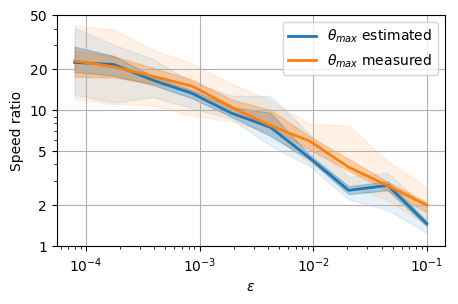
\includegraphics[scale=0.5]{images/speedratio_image}
                    \subcaption{Quadratic cost, random marginals}\label{fig:compare_a}
\end{minipage}%
			\begin{minipage}[b]{.5\linewidth}
                    \centering
			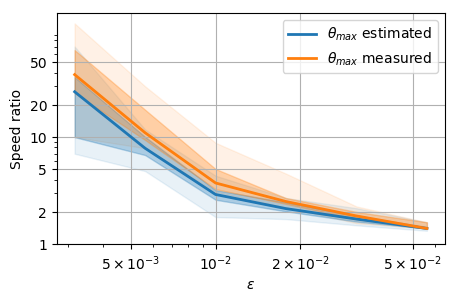
\includegraphics[scale=0.5]{images/speedratio_ML}
                    \subcaption{Random cost, uniform marginals}\label{fig:compare_b}
\end{minipage}
			\caption{\label{fig:comparison}Complexity ratio of SK algorithm and its accelerated version Algorithm~\ref{SOR}.}% (stopping criterion $\Vert u - u^* \Vert_\infty<10^{-6})$
\end{figure}


\section{Conclusion and perspectives}
SK algorithm is widely used to solve entropy regularized OT. The use of overrelaxed projections turns out to be a natural and simple idea to accelerate convergence while keeping many nice properties of this algorithm (first order, paralelizable, simple). We have proposed an algorithm that adaptively chooses the overrelaxation parameter so as to guarantee global convergence. The acceleration of the convergence speed is numerically impressive, in particular in low regularization regimes. It is theoretically supported in the local regime by the standard analysis of SOR iterations.

This idea of overrelaxation can be generalized to solve more general problems such as barycenters, gradient flows, unbalanced OT~\cite[chap. 4]{chizat2017these} but there is no systematic way to derive globally convergent algorithms. Our work as an effort in the direction of building and understanding the properties of robust first order algorithms for solving OT. More understanding is needed regarding SOR itself (global convergence speed, choice of $\theta_0$), but also its relation to other acceleration methods~\cite{2016arXiv160604133S,2017arXiv170509634A}.

%Links with monotone Fista? (that choose Fista if energy decreased and forward backward otherwise...)





\section*{Acknowledgments}
This study has been carried out with financial support from the French State, managed by the French National Research Agency (ANR) in the frame of the  GOTMI project (ANR-16-CE33-0010-01).

%\subsubsection*{References}

\bibliographystyle{apalike}
\bibliography{references}

\end{document}
=======
\documentclass{article} % For LaTeX2e
\usepackage{nips14submit_e,times}
\usepackage{hyperref}
\usepackage{url}
\usepackage{amsmath}
\usepackage{amssymb}
\usepackage{amsthm}
\usepackage{mathtools,enumitem}
\usepackage{algorithm}
\usepackage{algorithmic}
%\documentstyle[nips14submit_09,times,art10]{article} % For LaTeX 2.09

\usepackage{tikz}
\usepackage{cite}

% Math operators
\newcommand{\scal}[2]{\left\langle #1 , #2 \right\rangle}
\DeclareMathOperator{\IR}{\mathbb{R}}
\DeclareMathOperator*{\argmin}{argmin}
\DeclareMathOperator{\One}{\mathbbm{1}}
\DeclareMathOperator{\Ccal}{\mathcal{C}}
\DeclareMathOperator{\logsumexp}{logsumexp}
\DeclareMathOperator{\diag}{diag}
\newcommand{\norm}[1]{\left\lVert #1 \right\rVert}
\renewcommand{\epsilon}{\varepsilon}

\theoremstyle{plain}
\newtheorem{theorem}{Theorem}
\newtheorem{proposition}{Proposition}
\newtheorem{lemma}{Lemma}
\newtheorem{corollary}{Corollary}

\theoremstyle{definition}
\newtheorem{definition}{Definition}

\theoremstyle{remark}
\newtheorem{remark}{Remark}
\newtheorem{example}{Example}


\title{Over-relaxed Sinkhorn--Knopp Algorithm for Regularized Optimal Transport}

%
\author{
Alexis THIBAULT\\
\'Ecole Normale Sup\'erieure\\
Paris, France\\
\texttt{alexis.thibault@ens.fr}
 \And
L\'enaic CHIZAT\\
\'Ecole Normale Sup\'erieure\\ Paris Dauphine (PSL research University)\\
Paris, France\\
\texttt{lenaic.chizat@ens.fr}
 \AND
Charles DOSSAL\\
INSA Toulouse\\
Institut de Math\'ematiques de Toulouse\\
Toulouse,  France\\
\texttt{dossal@insa-toulouse.fr}
\And 
Nicolas PAPADAKIS\\
CNRS, Institut de Math\'ematiques de Bordeaux\\
Talence, France\\
\texttt{nicolas.papadakis@math.u-bordeaux.fr}
} 
% The \author macro works with any number of authors. There are two commands
% used to separate the names and addresses of multiple authors: \And and \AND.
%
% Using \And between authors leaves it to \LaTeX{} to determine where to break
% the lines. Using \AND forces a linebreak at that point. So, if \LaTeX{}
% puts 3 of 4 authors names on the first line, and the last on the second
% line, try using \AND instead of \And before the third author name.

\newcommand{\fix}{\marginpar{FIX}}
\newcommand{\new}{\marginpar{NEW}}

\nipsfinalcopy % Uncomment for camera-ready version

\begin{document}


\maketitle

\begin{abstract}
This article describes a method for quickly calculating the solution to the regularized optimal transport problem. It generalizes and improves upon the widely-used iterative Bregman projections algorithm (or Sinkhorn--Knopp algorithm). 
The idea is to over-relax the Bregman projection operators, allowing for faster convergence. In practice this corresponds to elevating the diagonal scaling factors to a given power, at each step of the algorithm.
In this paper, we propose a simple method for establishing the global convergence of the over-relaxed Sinkhorn--Knopp algorithm, by ensuring the decrease of a Lyapunov function at each step.
An inexpensive adaptive choice of over-relaxation parameter based on the Lyapunov function is constructed.
We also suggest a heuristic to choose a suitable asymptotic over-relaxation parameter.
\end{abstract}

\section{Introduction}
Optimal Transport is an efficient and flexible tool to compare two probability distributions which has been popularized in the computer vision community in the context of discrete histograms \cite{Rubner2000}. The introduction of entropic regularization in \cite{cuturi13} has made possible the use of the fast Sinkhorn--Knopp algorithm \cite{sinkhorn64}   scaling with high dimensional data. 
Regularized optimal transport have thus been intensively used  in  Machine Learning with applications such as   Geodesic PCA \cite{seguy2015principal}, domain adaptation \cite{2015arXiv150700504C}, data fitting \cite{2015arXiv150605439F},  training of Boltzmann Machine \cite{NIPS2016_6248}  or dictionary learning \cite{Rolet2016,2017arXiv170801955S}.

The computation of optimal transport between two data relies on the estimation of an optimal transport matrix, the entries of which represent the quantity of mass transported between  data locations. 
Regularization of optimal transport with strictly convex regularizers \cite{cuturi13, dessein2016}  nevertheless involves a spreading of the mass. Hence, for particular purposes such as color interpolation \cite{Rabin2014} or gradient flow \cite{2016arXiv160705816C}, it is  necessary  to consider very small regularization of the problem.
In this setting,  the regularized transport problem can be ill-conditioned, rendering the Sinkhorn--Knopp algorithm significantly slower. This is the issue  we want to tackle here.
Before going into further details, we now briefly introduce the main notations and concepts used all along this article.

 
\subsection{Discrete Optimal Transport}
We consider two discrete probability measures $\mu^k \in \IR_{+*}^{n_k}$.
Let us define the two following linear operators
\begin{align*}
A_1 &: \begin{cases}
\IR^{n_1 n_2} \rightarrow \IR^{n_1} \\
(A_1 x)_i = \sum_j x_{i,j}
\end{cases} &
A_2 &: \begin{cases}
\IR^{n_1 n_2} \rightarrow \IR^{n_2}\\
(A_2 x)_j = \sum_i x_{i,j},
\end{cases}
\end{align*}
as well as the linear  constraint sets
\begin{align*}
\Ccal_k &= \left\{ \gamma\in\IR^{n_1 n_2} \mid A_k \gamma = \mu^k \right\}.
\end{align*}
Given a cost matrix $c$, where $c_{ij}$ represents the cost of moving mass $\mu^1_i$ to $\mu^2_j$,  the optimal transport problem corresponds to the estimation of an optimal transport matrix $\gamma$ solution of:
$$\min_{\gamma\in\Ccal_1\cap \Ccal_2\cap \IR^{n_1 n_2}_+} \langle c,\gamma\rangle:=\sum_{i,j}c_{i,j}\gamma_{i,j}.$$
This is a linear programing problem whose resolution is unmanageable for large scale problems. 

\subsection{Regularized optimal transport}

In \cite{cuturi13}, it has been proposed to regularize this problem by adding a strictly convex entropy regularization:
\begin{equation}\label{ROT}
\min_{\gamma\in\Ccal_1\cap \Ccal_2\cap \IR^{n_1 n_2}_{+*}}K^\epsilon(\gamma) := \scal{c}{\gamma} 
+ \epsilon KL(\gamma,\mathbf{1})
,\end{equation}
with $\epsilon>0$, $\mathbf{1}$ is the matrix of size $n_1\times n_2$ full of ones and the Kullback-Leibler divergence is:
\begin{equation}\label{KL}
KL(\gamma,\xi) = \sum_{i,j} \gamma_{i,j} \left( \log \left( \frac{\gamma_{i,j}}{\xi_{i,j}} \right) -1  \right) + \sum_{i,j} \xi_{i,j}.
\end{equation}
It was shown in \cite{benamou15}  that the regularized optimal transport matrix $\gamma^*$, which is the unique minimizer of problem \eqref{ROT},  is the Bregman projection of $\gamma^0 = e^{-c/\epsilon}$ onto $\Ccal_1 \cap \Ccal_2$:
\begin{equation}\label{eq:reg_ot_pb}
\gamma^* = \argmin_{\Ccal_1 \cap \Ccal_2} K^\epsilon(\gamma)= P_{\Ccal_1 \cap \Ccal_2} (e^{-c/\epsilon}),
\end{equation}
where $P_{\Ccal}$ is the  Bregman projection onto $\Ccal$ defined as:
\begin{equation}\label{eq:P_C}
P_{\Ccal}(\xi) := \argmin_{\gamma \in \Ccal} KL(\gamma,\xi).
\end{equation}



\subsection{The Sinkhorn--Knopp algorithm}
Iterative Bregman projections onto $\Ccal_1$ and $\Ccal_2$ converge to a point in the intersection $\Ccal_1 \cap \Ccal_2$ \cite{bregman67}. Hence, the so-called Sinkhorn--Knopp algorithm \cite{sinkhorn64} that performs alternate Bregman projections, can be considered to compute the regularized  transport matrix:
\begin{align*}
\gamma^0 &= e^{-c/\epsilon} &
\gamma^{l+1} = P_{\Ccal_2}(P_{\Ccal_1}(\gamma^l)),
\end{align*}
and we have 
$\lim_{l\rightarrow +\infty} \gamma^l = P_{\Ccal_1 \cap \Ccal_2}(\gamma^0) = \gamma^*.$

In the discrete setting,  projections actually correspond to diagonal scalings. This can be seen by writing the minimality conditions for the projection, given equations (\ref{KL}) and (\ref{eq:P_C}).
\begin{align}\label{scaling}
P_{\Ccal_1}(\gamma) &= \diag(a) \gamma &
a &=  {\mu^1}\oslash{A_1 \gamma} \\
P_{\Ccal_2}(\gamma) &= \gamma \diag(b) &
b &= {\mu^2}\oslash{A_2 \gamma}\nonumber
\end{align}
where $\oslash$ is the pointwise division. 
To compute numerically the solution  one simply has to store $(a^l, b^l)\in\IR^{n_1+n_2}$ and to iterate
\begin{align*}
a^{l+1} &= {\mu^1}\oslash{\gamma^0 b^l} &
b^{l+1} &= {\mu^2}\oslash{^t \gamma^0 a^{l+1}} 
\end{align*}
where the transport matrix can be recovered as :
$\gamma^l = \diag(a^l) \gamma^0 \diag(b^l).$ 
Efficient parallel computations can be considered \cite{cuturi13} and one can even reach real-time computation for large scale problem for certain class of cost matrices $c$ \cite{Solomon2015}. 
For small values of the parameter $\epsilon$, numerical issues can arise and a stabilization of the algorithm is necessary \cite{2016arXiv160705816C}.
The convergence of the process can nevertheless be very slow  in the setting $\epsilon\to 0$.
\subsection{Related works }
The introduction of relaxation variables through heavy ball approaches \cite{POLYAK19641} has recently gained in popularity  to speed up the convergence of algorithms optimizing convex \cite{2014arXiv1412.7457G} or non convex \cite{Zavriev1993,2016arXiv160609070O} problems. Such schemes have also been empirically considered to accelerate the SK algorithm  in \cite{peyre2016quantum,2017arXiv170801955S}. The convergence of these algorithms is nevertheless not studied yet in the context of regularized optimal transport.

\subsection{Overview and contributions}
In this paper, we consider an over-relaxation scheme designed to accelerate the Sinkhorn--Knopp algorithm. We first present and show the convergence of our algorithm in section 2. In section 3, we analyze the local convergence rate of the algorithm to justify the acceleration.
We finally demonstrate numerically  in Section 4 the good behavior of our method, where larger accelerations are observed for decreasing values of $\epsilon$.



\section{Over-relaxed Sinkhorn--Knopp algorithm}

As illustrated in Figure \ref{alternate_projections} (a-b), the SK algorithm, that  performs alternate Bregman projections onto the affine sets $\Ccal_1$ and $\Ccal_2$, can be very slow when $\epsilon\to 0$, as the problem becomes ill-conditioned. The idea developped in this paper is to perform over-relaxed projections in order to accelerate the process, as displayed in Figure \ref{alternate_projections} (c).

\begin{figure}[ht!]
\begin{center}
\begin{tabular}{ccc}
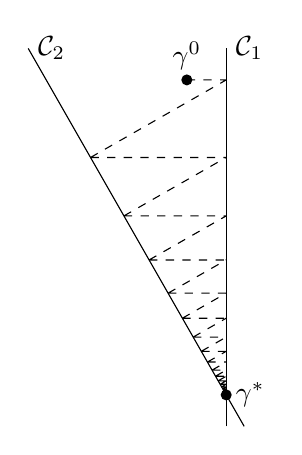
\begin{tikzpicture}
\fill (-0.500000,4.000000) circle (2pt) node[above] (gamma0) {$\gamma^0$};
\fill (0,0) circle (2pt) node[right] {$\gamma^*$};
\draw[dashed] (-0.500000,4.000000) -- (0.000000,4.000000)
(-1.723077,3.015385) -- (0.000000,4.000000)
(-1.723077,3.015385) -- (0.000000,3.015385)
(-1.298935,2.273136) -- (0.000000,3.015385)
(-1.298935,2.273136) -- (0.000000,2.273136)
(-0.979197,1.713595) -- (0.000000,2.273136)
(-0.979197,1.713595) -- (0.000000,1.713595)
(-0.738164,1.291787) -- (0.000000,1.713595)
(-0.738164,1.291787) -- (0.000000,1.291787)
(-0.556462,0.973809) -- (0.000000,1.291787)
(-0.556462,0.973809) -- (0.000000,0.973809)
(-0.419487,0.734102) -- (0.000000,0.973809)
(-0.419487,0.734102) -- (0.000000,0.734102)
(-0.316228,0.553400) -- (0.000000,0.734102)
(-0.316228,0.553400) -- (0.000000,0.553400)
(-0.238388,0.417178) -- (0.000000,0.553400)
(-0.238388,0.417178) -- (0.000000,0.417178)
(-0.179708,0.314488) -- (0.000000,0.417178)
(-0.179708,0.314488) -- (0.000000,0.314488)
(-0.135472,0.237076) -- (0.000000,0.314488)
(-0.135472,0.237076) -- (0.000000,0.237076)
(-0.102125,0.178719) -- (0.000000,0.237076)
(-0.102125,0.178719) -- (0.000000,0.178719)
(-0.076987,0.134726) -- (0.000000,0.178719)
(-0.076987,0.134726) -- (0.000000,0.134726)
(-0.058036,0.101563) -- (0.000000,0.134726)
(-0.058036,0.101563) -- (0.000000,0.101563)
(-0.043750,0.076563) -- (0.000000,0.101563)
(-0.043750,0.076563) -- (0.000000,0.076563)
(-0.032981,0.057717) -- (0.000000,0.076563)
(-0.032981,0.057717) -- (0.000000,0.057717)
(-0.024863,0.043509) -- (0.000000,0.057717)
(-0.024863,0.043509) -- (0.000000,0.043509)
(-0.018743,0.032799) -- (0.000000,0.043509)
(-0.018743,0.032799) -- (0.000000,0.032799)
(-0.014129,0.024726) -- (0.000000,0.032799)
(-0.014129,0.024726) -- (0.000000,0.024726)
(-0.010651,0.018639) -- (0.000000,0.024726)
(-0.010651,0.018639) -- (0.000000,0.018639)
(-0.008029,0.014051) -- (0.000000,0.018639)
(-0.008029,0.014051) -- (0.000000,0.014051)
(-0.006053,0.010592) -- (0.000000,0.014051)
(-0.006053,0.010592) -- (0.000000,0.010592)
(-0.004563,0.007985) -- (0.000000,0.010592)
(-0.004563,0.007985) -- (0.000000,0.007985)
(-0.003440,0.006020) -- (0.000000,0.007985)
(-0.003440,0.006020) -- (0.000000,0.006020)
(-0.002593,0.004538) -- (0.000000,0.006020)
(-0.002593,0.004538) -- (0.000000,0.004538)
(-0.001955,0.003421) -- (0.000000,0.004538)
(-0.001955,0.003421) -- (0.000000,0.003421)
(-0.001474,0.002579) -- (0.000000,0.003421)
(-0.001474,0.002579) -- (0.000000,0.002579)
(-0.001111,0.001944) -- (0.000000,0.002579)
(-0.001111,0.001944) -- (0.000000,0.001944)
(-0.000837,0.001465) -- (0.000000,0.001944)
(-0.000837,0.001465) -- (0.000000,0.001465)
(-0.000631,0.001105) -- (0.000000,0.001465)
(-0.000631,0.001105) -- (0.000000,0.001105)
(-0.000476,0.000833) -- (0.000000,0.001105)
(-0.000476,0.000833) -- (0.000000,0.000833)
(-0.000359,0.000628) -- (0.000000,0.000833)
(-0.000359,0.000628) -- (0.000000,0.000628)
(-0.000270,0.000473) -- (0.000000,0.000628)
(-0.000270,0.000473) -- (0.000000,0.000473)
(-0.000204,0.000357) -- (0.000000,0.000473)
(-0.000204,0.000357) -- (0.000000,0.000357)
(-0.000154,0.000269) -- (0.000000,0.000357)
(-0.000154,0.000269) -- (0.000000,0.000269)
(-0.000116,0.000203) -- (0.000000,0.000269)
(-0.000116,0.000203) -- (0.000000,0.000203)
(-0.000087,0.000153) -- (0.000000,0.000203)
(-0.000087,0.000153) -- (0.000000,0.000153)
(-0.000066,0.000115) -- (0.000000,0.000153)
(-0.000066,0.000115) -- (0.000000,0.000115)
(-0.000050,0.000087) -- (0.000000,0.000115)
(-0.000050,0.000087) -- (0.000000,0.000087)
(-0.000037,0.000065) -- (0.000000,0.000087)
(-0.000037,0.000065) -- (0.000000,0.000065)
(-0.000028,0.000049) -- (0.000000,0.000065)
(-0.000028,0.000049) -- (0.000000,0.000049)
(-0.000021,0.000037) -- (0.000000,0.000049)
(-0.000021,0.000037) -- (0.000000,0.000037)
(-0.000016,0.000028) -- (0.000000,0.000037)
(-0.000016,0.000028) -- (0.000000,0.000028)
(-0.000012,0.000021) -- (0.000000,0.000028)
(-0.000012,0.000021) -- (0.000000,0.000021)
(-0.000009,0.000016) -- (0.000000,0.000021)
(-0.000009,0.000016) -- (0.000000,0.000016)
(-0.000007,0.000012) -- (0.000000,0.000016)
(-0.000007,0.000012) -- (0.000000,0.000012)
(-0.000005,0.000009) -- (0.000000,0.000012)
(-0.000005,0.000009) -- (0.000000,0.000009)
(-0.000004,0.000007) -- (0.000000,0.000009)
(-0.000004,0.000007) -- (0.000000,0.000007)
(-0.000003,0.000005) -- (0.000000,0.000007)
(-0.000003,0.000005) -- (0.000000,0.000005)
(-0.000002,0.000004) -- (0.000000,0.000005)
(-0.000002,0.000004) -- (0.000000,0.000004)
(-0.000002,0.000003) -- (0.000000,0.000004)
(-0.000002,0.000003) -- (0.000000,0.000003)
(-0.000001,0.000002) -- (0.000000,0.000003)
(-0.000001,0.000002) -- (0.000000,0.000002)
(-0.000001,0.000002) -- (0.000000,0.000002)
(-0.000001,0.000002) -- (0.000000,0.000002)
(-0.000001,0.000001) -- (0.000000,0.000002)
(-0.000001,0.000001) -- (0.000000,0.000001)
(-0.000001,0.000001) -- (0.000000,0.000001)
(-0.000001,0.000001) -- (0.000000,0.000001)
(-0.000000,0.000001) -- (0.000000,0.000001)
(-0.000000,0.000001) -- (0.000000,0.000001)
(-0.000000,0.000001) -- (0.000000,0.000001)
(-0.000000,0.000001) -- (0.000000,0.000001)
(-0.000000,0.000000) -- (0.000000,0.000001)
(-0.000000,0.000000) -- (0.000000,0.000000)
(-0.000000,0.000000) -- (0.000000,0.000000)
(-0.000000,0.000000) -- (0.000000,0.000000)
(-0.000000,0.000000) -- (0.000000,0.000000)
(-0.000000,0.000000) -- (0.000000,0.000000)
(-0.000000,0.000000) -- (0.000000,0.000000)
(-0.000000,0.000000) -- (0.000000,0.000000)
(-0.000000,0.000000) -- (0.000000,0.000000)
(-0.000000,0.000000) -- (0.000000,0.000000)
(-0.000000,0.000000) -- (0.000000,0.000000)
(-0.000000,0.000000) -- (0.000000,0.000000)
(-0.000000,0.000000) -- (0.000000,0.000000)
(-0.000000,0.000000) -- (0.000000,0.000000)
(-0.000000,0.000000) -- (0.000000,0.000000)
(-0.000000,0.000000) -- (0.000000,0.000000)
(-0.000000,0.000000) -- (0.000000,0.000000)
(-0.000000,0.000000) -- (0.000000,0.000000)
(-0.000000,0.000000) -- (0.000000,0.000000)
(-0.000000,0.000000) -- (0.000000,0.000000)
(-0.000000,0.000000) -- (0.000000,0.000000)
(-0.000000,0.000000) -- (0.000000,0.000000)
(-0.000000,0.000000) -- (0.000000,0.000000)
(-0.000000,0.000000) -- (0.000000,0.000000)
(-0.000000,0.000000) -- (0.000000,0.000000)
(-0.000000,0.000000) -- (0.000000,0.000000)
(-0.000000,0.000000) -- (0.000000,0.000000)
(-0.000000,0.000000) -- (0.000000,0.000000)
(-0.000000,0.000000) -- (0.000000,0.000000)
(-0.000000,0.000000) -- (0.000000,0.000000)
(-0.000000,0.000000) -- (0.000000,0.000000)
(-0.000000,0.000000) -- (0.000000,0.000000)
(-0.000000,0.000000) -- (0.000000,0.000000)
(-0.000000,0.000000) -- (0.000000,0.000000)
(-0.000000,0.000000) -- (0.000000,0.000000)
(-0.000000,0.000000) -- (0.000000,0.000000)
(-0.000000,0.000000) -- (0.000000,0.000000)
(-0.000000,0.000000) -- (0.000000,0.000000)
(-0.000000,0.000000) -- (0.000000,0.000000)
(-0.000000,0.000000) -- (0.000000,0.000000)
(-0.000000,0.000000) -- (0.000000,0.000000)
(-0.000000,0.000000) -- (0.000000,0.000000)
(-0.000000,0.000000) -- (0.000000,0.000000)
(-0.000000,0.000000) -- (0.000000,0.000000)
(-0.000000,0.000000) -- (0.000000,0.000000)
(-0.000000,0.000000) -- (0.000000,0.000000)
(-0.000000,0.000000) -- (0.000000,0.000000)
(-0.000000,0.000000) -- (0.000000,0.000000)
(-0.000000,0.000000) -- (0.000000,0.000000)
(-0.000000,0.000000) -- (0.000000,0.000000)
(-0.000000,0.000000) -- (0.000000,0.000000)
(-0.000000,0.000000) -- (0.000000,0.000000)
(-0.000000,0.000000) -- (0.000000,0.000000)
(-0.000000,0.000000) -- (0.000000,0.000000)
(-0.000000,0.000000) -- (0.000000,0.000000)
(-0.000000,0.000000) -- (0.000000,0.000000)
(-0.000000,0.000000) -- (0.000000,0.000000)
(-0.000000,0.000000) -- (0.000000,0.000000)
(-0.000000,0.000000) -- (0.000000,0.000000)
(-0.000000,0.000000) -- (0.000000,0.000000)
(-0.000000,0.000000) -- (0.000000,0.000000)
(-0.000000,0.000000) -- (0.000000,0.000000)
(-0.000000,0.000000) -- (0.000000,0.000000)
(-0.000000,0.000000) -- (0.000000,0.000000)
(-0.000000,0.000000) -- (0.000000,0.000000)
(-0.000000,0.000000) -- (0.000000,0.000000)
(-0.000000,0.000000) -- (0.000000,0.000000)
(-0.000000,0.000000) -- (0.000000,0.000000)
(-0.000000,0.000000) -- (0.000000,0.000000)
(-0.000000,0.000000) -- (0.000000,0.000000)
(-0.000000,0.000000) -- (0.000000,0.000000)
(-0.000000,0.000000) -- (0.000000,0.000000)
(-0.000000,0.000000) -- (0.000000,0.000000)
(-0.000000,0.000000) -- (0.000000,0.000000)
(-0.000000,0.000000) -- (0.000000,0.000000)
(-0.000000,0.000000) -- (0.000000,0.000000)
(-0.000000,0.000000) -- (0.000000,0.000000)
(-0.000000,0.000000) -- (0.000000,0.000000)
(-0.000000,0.000000) -- (0.000000,0.000000)
(-0.000000,0.000000) -- (0.000000,0.000000)
(-0.000000,0.000000) -- (0.000000,0.000000)
(-0.000000,0.000000) -- (0.000000,0.000000)
(-0.000000,0.000000) -- (0.000000,0.000000)
(-0.000000,0.000000) -- (0.000000,0.000000)
(-0.000000,0.000000) -- (0.000000,0.000000)
(-0.000000,0.000000) -- (0.000000,0.000000)
(-0.000000,0.000000) -- (0.000000,0.000000)
;
\draw (-0.000000,-0.400000) -- (0.000000,4.400000) node[right] {$\mathcal{C}_1$};
\draw (0.228571,-0.400000) -- (-2.514286,4.400000) node[right] {$\mathcal{C}_2$};
\end{tikzpicture}
&
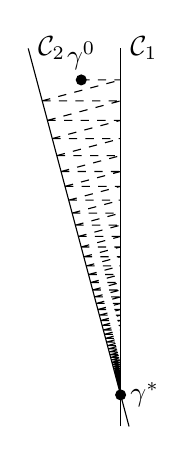
\begin{tikzpicture}
\fill (-0.500000,4.000000) circle (2pt) node[above] (gamma0) {$\gamma^0$};
\fill (0,0) circle (2pt) node[right] {$\gamma^*$};
\draw[dashed] (-0.500000,4.000000) -- (0.000000,4.000000)
(-0.995851,3.734440) -- (0.000000,4.000000)
(-0.995851,3.734440) -- (0.000000,3.734440)
(-0.929736,3.486510) -- (0.000000,3.734440)
(-0.929736,3.486510) -- (0.000000,3.486510)
(-0.868011,3.255041) -- (0.000000,3.486510)
(-0.868011,3.255041) -- (0.000000,3.255041)
(-0.810384,3.038938) -- (0.000000,3.255041)
(-0.810384,3.038938) -- (0.000000,3.038938)
(-0.756582,2.837183) -- (0.000000,3.038938)
(-0.756582,2.837183) -- (0.000000,2.837183)
(-0.706353,2.648822) -- (0.000000,2.837183)
(-0.706353,2.648822) -- (0.000000,2.648822)
(-0.659458,2.472967) -- (0.000000,2.648822)
(-0.659458,2.472967) -- (0.000000,2.472967)
(-0.615676,2.308787) -- (0.000000,2.472967)
(-0.615676,2.308787) -- (0.000000,2.308787)
(-0.574802,2.155506) -- (0.000000,2.308787)
(-0.574802,2.155506) -- (0.000000,2.155506)
(-0.536641,2.012402) -- (0.000000,2.155506)
(-0.536641,2.012402) -- (0.000000,2.012402)
(-0.501013,1.878799) -- (0.000000,2.012402)
(-0.501013,1.878799) -- (0.000000,1.878799)
(-0.467751,1.754065) -- (0.000000,1.878799)
(-0.467751,1.754065) -- (0.000000,1.754065)
(-0.436697,1.637613) -- (0.000000,1.754065)
(-0.436697,1.637613) -- (0.000000,1.637613)
(-0.407704,1.528891) -- (0.000000,1.637613)
(-0.407704,1.528891) -- (0.000000,1.528891)
(-0.380637,1.427388) -- (0.000000,1.528891)
(-0.380637,1.427388) -- (0.000000,1.427388)
(-0.355366,1.332624) -- (0.000000,1.427388)
(-0.355366,1.332624) -- (0.000000,1.332624)
(-0.331774,1.244151) -- (0.000000,1.332624)
(-0.331774,1.244151) -- (0.000000,1.244151)
(-0.309747,1.161552) -- (0.000000,1.244151)
(-0.309747,1.161552) -- (0.000000,1.161552)
(-0.289183,1.084436) -- (0.000000,1.161552)
(-0.289183,1.084436) -- (0.000000,1.084436)
(-0.269984,1.012440) -- (0.000000,1.084436)
(-0.269984,1.012440) -- (0.000000,1.012440)
(-0.252060,0.945225) -- (0.000000,1.012440)
(-0.252060,0.945225) -- (0.000000,0.945225)
(-0.235326,0.882471) -- (0.000000,0.945225)
(-0.235326,0.882471) -- (0.000000,0.882471)
(-0.219702,0.823884) -- (0.000000,0.882471)
(-0.219702,0.823884) -- (0.000000,0.823884)
(-0.205116,0.769186) -- (0.000000,0.823884)
(-0.205116,0.769186) -- (0.000000,0.769186)
(-0.191499,0.718120) -- (0.000000,0.769186)
(-0.191499,0.718120) -- (0.000000,0.718120)
(-0.178785,0.670444) -- (0.000000,0.718120)
(-0.178785,0.670444) -- (0.000000,0.670444)
(-0.166915,0.625933) -- (0.000000,0.670444)
(-0.166915,0.625933) -- (0.000000,0.625933)
(-0.155834,0.584377) -- (0.000000,0.625933)
(-0.155834,0.584377) -- (0.000000,0.584377)
(-0.145488,0.545580) -- (0.000000,0.584377)
(-0.145488,0.545580) -- (0.000000,0.545580)
(-0.135829,0.509359) -- (0.000000,0.545580)
(-0.135829,0.509359) -- (0.000000,0.509359)
(-0.126811,0.475543) -- (0.000000,0.509359)
(-0.126811,0.475543) -- (0.000000,0.475543)
(-0.118392,0.443972) -- (0.000000,0.475543)
(-0.118392,0.443972) -- (0.000000,0.443972)
(-0.110532,0.414496) -- (0.000000,0.443972)
(-0.110532,0.414496) -- (0.000000,0.414496)
(-0.103194,0.386978) -- (0.000000,0.414496)
(-0.103194,0.386978) -- (0.000000,0.386978)
(-0.096343,0.361286) -- (0.000000,0.386978)
(-0.096343,0.361286) -- (0.000000,0.361286)
(-0.089947,0.337301) -- (0.000000,0.361286)
(-0.089947,0.337301) -- (0.000000,0.337301)
(-0.083975,0.314907) -- (0.000000,0.337301)
(-0.083975,0.314907) -- (0.000000,0.314907)
(-0.078400,0.294000) -- (0.000000,0.314907)
(-0.078400,0.294000) -- (0.000000,0.294000)
(-0.073195,0.274482) -- (0.000000,0.294000)
(-0.073195,0.274482) -- (0.000000,0.274482)
(-0.068336,0.256259) -- (0.000000,0.274482)
(-0.068336,0.256259) -- (0.000000,0.256259)
(-0.063799,0.239246) -- (0.000000,0.256259)
(-0.063799,0.239246) -- (0.000000,0.239246)
(-0.059563,0.223362) -- (0.000000,0.239246)
(-0.059563,0.223362) -- (0.000000,0.223362)
(-0.055609,0.208533) -- (0.000000,0.223362)
(-0.055609,0.208533) -- (0.000000,0.208533)
(-0.051917,0.194689) -- (0.000000,0.208533)
(-0.051917,0.194689) -- (0.000000,0.194689)
(-0.048470,0.181763) -- (0.000000,0.194689)
(-0.048470,0.181763) -- (0.000000,0.181763)
(-0.045252,0.169696) -- (0.000000,0.181763)
(-0.045252,0.169696) -- (0.000000,0.169696)
(-0.042248,0.158430) -- (0.000000,0.169696)
(-0.042248,0.158430) -- (0.000000,0.158430)
(-0.039443,0.147912) -- (0.000000,0.158430)
(-0.039443,0.147912) -- (0.000000,0.147912)
(-0.036825,0.138092) -- (0.000000,0.147912)
(-0.036825,0.138092) -- (0.000000,0.138092)
(-0.034380,0.128924) -- (0.000000,0.138092)
(-0.034380,0.128924) -- (0.000000,0.128924)
(-0.032097,0.120365) -- (0.000000,0.128924)
(-0.032097,0.120365) -- (0.000000,0.120365)
(-0.029966,0.112374) -- (0.000000,0.120365)
(-0.029966,0.112374) -- (0.000000,0.112374)
(-0.027977,0.104913) -- (0.000000,0.112374)
(-0.027977,0.104913) -- (0.000000,0.104913)
(-0.026119,0.097948) -- (0.000000,0.104913)
(-0.026119,0.097948) -- (0.000000,0.097948)
(-0.024385,0.091445) -- (0.000000,0.097948)
(-0.024385,0.091445) -- (0.000000,0.091445)
(-0.022766,0.085374) -- (0.000000,0.091445)
(-0.022766,0.085374) -- (0.000000,0.085374)
(-0.021255,0.079706) -- (0.000000,0.085374)
(-0.021255,0.079706) -- (0.000000,0.079706)
(-0.019844,0.074415) -- (0.000000,0.079706)
(-0.019844,0.074415) -- (0.000000,0.074415)
(-0.018526,0.069474) -- (0.000000,0.074415)
(-0.018526,0.069474) -- (0.000000,0.069474)
(-0.017296,0.064862) -- (0.000000,0.069474)
(-0.017296,0.064862) -- (0.000000,0.064862)
(-0.016148,0.060556) -- (0.000000,0.064862)
(-0.016148,0.060556) -- (0.000000,0.060556)
(-0.015076,0.056535) -- (0.000000,0.060556)
(-0.015076,0.056535) -- (0.000000,0.056535)
(-0.014075,0.052782) -- (0.000000,0.056535)
(-0.014075,0.052782) -- (0.000000,0.052782)
(-0.013141,0.049278) -- (0.000000,0.052782)
(-0.013141,0.049278) -- (0.000000,0.049278)
(-0.012268,0.046006) -- (0.000000,0.049278)
(-0.012268,0.046006) -- (0.000000,0.046006)
(-0.011454,0.042952) -- (0.000000,0.046006)
(-0.011454,0.042952) -- (0.000000,0.042952)
(-0.010693,0.040100) -- (0.000000,0.042952)
(-0.010693,0.040100) -- (0.000000,0.040100)
(-0.009983,0.037438) -- (0.000000,0.040100)
(-0.009983,0.037438) -- (0.000000,0.037438)
(-0.009321,0.034952) -- (0.000000,0.037438)
(-0.009321,0.034952) -- (0.000000,0.034952)
(-0.008702,0.032632) -- (0.000000,0.034952)
(-0.008702,0.032632) -- (0.000000,0.032632)
(-0.008124,0.030466) -- (0.000000,0.032632)
(-0.008124,0.030466) -- (0.000000,0.030466)
(-0.007585,0.028443) -- (0.000000,0.030466)
(-0.007585,0.028443) -- (0.000000,0.028443)
(-0.007081,0.026555) -- (0.000000,0.028443)
(-0.007081,0.026555) -- (0.000000,0.026555)
(-0.006611,0.024792) -- (0.000000,0.026555)
(-0.006611,0.024792) -- (0.000000,0.024792)
(-0.006172,0.023146) -- (0.000000,0.024792)
(-0.006172,0.023146) -- (0.000000,0.023146)
(-0.005762,0.021609) -- (0.000000,0.023146)
(-0.005762,0.021609) -- (0.000000,0.021609)
(-0.005380,0.020174) -- (0.000000,0.021609)
(-0.005380,0.020174) -- (0.000000,0.020174)
(-0.005023,0.018835) -- (0.000000,0.020174)
(-0.005023,0.018835) -- (0.000000,0.018835)
(-0.004689,0.017585) -- (0.000000,0.018835)
(-0.004689,0.017585) -- (0.000000,0.017585)
(-0.004378,0.016417) -- (0.000000,0.017585)
(-0.004378,0.016417) -- (0.000000,0.016417)
(-0.004087,0.015327) -- (0.000000,0.016417)
(-0.004087,0.015327) -- (0.000000,0.015327)
(-0.003816,0.014310) -- (0.000000,0.015327)
(-0.003816,0.014310) -- (0.000000,0.014310)
(-0.003563,0.013360) -- (0.000000,0.014310)
(-0.003563,0.013360) -- (0.000000,0.013360)
(-0.003326,0.012473) -- (0.000000,0.013360)
(-0.003326,0.012473) -- (0.000000,0.012473)
(-0.003105,0.011645) -- (0.000000,0.012473)
(-0.003105,0.011645) -- (0.000000,0.011645)
(-0.002899,0.010872) -- (0.000000,0.011645)
(-0.002899,0.010872) -- (0.000000,0.010872)
(-0.002707,0.010150) -- (0.000000,0.010872)
(-0.002707,0.010150) -- (0.000000,0.010150)
(-0.002527,0.009476) -- (0.000000,0.010150)
(-0.002527,0.009476) -- (0.000000,0.009476)
(-0.002359,0.008847) -- (0.000000,0.009476)
(-0.002359,0.008847) -- (0.000000,0.008847)
(-0.002203,0.008259) -- (0.000000,0.008847)
(-0.002203,0.008259) -- (0.000000,0.008259)
(-0.002056,0.007711) -- (0.000000,0.008259)
(-0.002056,0.007711) -- (0.000000,0.007711)
(-0.001920,0.007199) -- (0.000000,0.007711)
(-0.001920,0.007199) -- (0.000000,0.007199)
(-0.001792,0.006721) -- (0.000000,0.007199)
(-0.001792,0.006721) -- (0.000000,0.006721)
(-0.001673,0.006275) -- (0.000000,0.006721)
(-0.001673,0.006275) -- (0.000000,0.006275)
(-0.001562,0.005858) -- (0.000000,0.006275)
(-0.001562,0.005858) -- (0.000000,0.005858)
(-0.001459,0.005469) -- (0.000000,0.005858)
(-0.001459,0.005469) -- (0.000000,0.005469)
(-0.001362,0.005106) -- (0.000000,0.005469)
(-0.001362,0.005106) -- (0.000000,0.005106)
(-0.001271,0.004767) -- (0.000000,0.005106)
(-0.001271,0.004767) -- (0.000000,0.004767)
(-0.001187,0.004451) -- (0.000000,0.004767)
(-0.001187,0.004451) -- (0.000000,0.004451)
(-0.001108,0.004155) -- (0.000000,0.004451)
;
\draw (-0.000000,-0.400000) -- (0.000000,4.400000) node[right] {$\mathcal{C}_1$};
\draw (0.106667,-0.400000) -- (-1.173333,4.400000) node[right] {$\mathcal{C}_2$};
\end{tikzpicture}
&
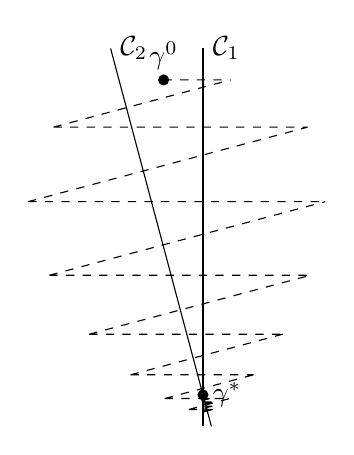
\begin{tikzpicture}
\fill (-0.500000,4.000000) circle (2pt) node[above] (gamma0) {$\gamma^0$};
\fill (0,0) circle (2pt) node[right] {$\gamma^*$};
\draw[dashed] (-0.500000,4.000000) -- (0.350000,4.000000)
(-1.898444,3.400415) -- (0.350000,4.000000)
(-1.898444,3.400415) -- (1.328911,3.400415)
(-2.219432,2.454190) -- (1.328911,3.400415)
(-2.219432,2.454190) -- (1.553603,2.454190)
(-1.950880,1.519661) -- (1.553603,2.454190)
(-1.950880,1.519661) -- (1.365616,1.519661)
(-1.444980,0.770169) -- (1.365616,1.519661)
(-1.444980,0.770169) -- (1.011486,0.770169)
(-0.919844,0.255148) -- (1.011486,0.770169)
(-0.919844,0.255148) -- (0.643891,0.255148)
(-0.486040,-0.046167) -- (0.643891,0.255148)
(-0.486040,-0.046167) -- (0.340228,-0.046167)
(-0.180221,-0.184954) -- (0.340228,-0.046167)
(-0.180221,-0.184954) -- (0.126154,-0.184954)
(0.004209,-0.217472) -- (0.126154,-0.184954)
(0.004209,-0.217472) -- (-0.002946,-0.217472)
(0.093772,-0.191681) -- (-0.002946,-0.217472)
(0.093772,-0.191681) -- (-0.065641,-0.191681)
(0.119666,-0.142266) -- (-0.065641,-0.191681)
(0.119666,-0.142266) -- (-0.083766,-0.142266)
(0.109394,-0.090756) -- (-0.083766,-0.142266)
(0.109394,-0.090756) -- (-0.076576,-0.090756)
(0.083372,-0.048103) -- (-0.076576,-0.090756)
(0.083372,-0.048103) -- (-0.058360,-0.048103)
(0.054625,-0.017974) -- (-0.058360,-0.048103)
(0.054625,-0.017974) -- (-0.038237,-0.017974)
(0.030058,0.000238) -- (-0.038237,-0.017974)
(0.030058,0.000238) -- (-0.021040,0.000238)
(0.012253,0.009116) -- (-0.021040,0.000238)
(0.012253,0.009116) -- (-0.008577,0.009116)
(0.001178,0.011717) -- (-0.008577,0.009116)
(0.001178,0.011717) -- (-0.000824,0.011717)
(-0.004475,0.010744) -- (-0.000824,0.011717)
(-0.004475,0.010744) -- (0.003133,0.010744)
(-0.006387,0.008205) -- (0.003133,0.010744)
(-0.006387,0.008205) -- (0.004471,0.008205)
(-0.006098,0.005387) -- (0.004471,0.008205)
(-0.006098,0.005387) -- (0.004268,0.005387)
(-0.004786,0.002973) -- (0.004268,0.005387)
(-0.004786,0.002973) -- (0.003350,0.002973)
(-0.003225,0.001219) -- (0.003350,0.002973)
(-0.003225,0.001219) -- (0.002258,0.001219)
(-0.001842,0.000126) -- (0.002258,0.001219)
(-0.001842,0.000126) -- (0.001289,0.000126)
(-0.000810,-0.000434) -- (0.001289,0.000126)
(-0.000810,-0.000434) -- (0.000567,-0.000434)
(-0.000149,-0.000625) -- (0.000567,-0.000434)
(-0.000149,-0.000625) -- (0.000105,-0.000625)
(0.000203,-0.000599) -- (0.000105,-0.000625)
(0.000203,-0.000599) -- (-0.000142,-0.000599)
(0.000337,-0.000471) -- (-0.000142,-0.000599)
(0.000337,-0.000471) -- (-0.000236,-0.000471)
(0.000338,-0.000318) -- (-0.000236,-0.000471)
(0.000338,-0.000318) -- (-0.000236,-0.000318)
(0.000273,-0.000182) -- (-0.000236,-0.000318)
(0.000273,-0.000182) -- (-0.000191,-0.000182)
(0.000189,-0.000080) -- (-0.000191,-0.000182)
(0.000189,-0.000080) -- (-0.000133,-0.000080)
(0.000112,-0.000015) -- (-0.000133,-0.000080)
(0.000112,-0.000015) -- (-0.000078,-0.000015)
(0.000052,0.000020) -- (-0.000078,-0.000015)
(0.000052,0.000020) -- (-0.000037,0.000020)
(0.000013,0.000033) -- (-0.000037,0.000020)
(0.000013,0.000033) -- (-0.000009,0.000033)
(-0.000008,0.000033) -- (-0.000009,0.000033)
(-0.000008,0.000033) -- (0.000006,0.000033)
(-0.000018,0.000027) -- (0.000006,0.000033)
(-0.000018,0.000027) -- (0.000012,0.000027)
(-0.000019,0.000019) -- (0.000012,0.000027)
(-0.000019,0.000019) -- (0.000013,0.000019)
(-0.000016,0.000011) -- (0.000013,0.000019)
(-0.000016,0.000011) -- (0.000011,0.000011)
(-0.000011,0.000005) -- (0.000011,0.000011)
(-0.000011,0.000005) -- (0.000008,0.000005)
(-0.000007,0.000001) -- (0.000008,0.000005)
(-0.000007,0.000001) -- (0.000005,0.000001)
(-0.000003,-0.000001) -- (0.000005,0.000001)
(-0.000003,-0.000001) -- (0.000002,-0.000001)
(-0.000001,-0.000002) -- (0.000002,-0.000001)
(-0.000001,-0.000002) -- (0.000001,-0.000002)
(0.000000,-0.000002) -- (0.000001,-0.000002)
(0.000000,-0.000002) -- (-0.000000,-0.000002)
(0.000001,-0.000002) -- (-0.000000,-0.000002)
(0.000001,-0.000002) -- (-0.000001,-0.000002)
(0.000001,-0.000001) -- (-0.000001,-0.000002)
(0.000001,-0.000001) -- (-0.000001,-0.000001)
(0.000001,-0.000001) -- (-0.000001,-0.000001)
(0.000001,-0.000001) -- (-0.000001,-0.000001)
(0.000001,-0.000000) -- (-0.000001,-0.000001)
(0.000001,-0.000000) -- (-0.000000,-0.000000)
(0.000000,-0.000000) -- (-0.000000,-0.000000)
(0.000000,-0.000000) -- (-0.000000,-0.000000)
(0.000000,0.000000) -- (-0.000000,-0.000000)
(0.000000,0.000000) -- (-0.000000,0.000000)
(0.000000,0.000000) -- (-0.000000,0.000000)
(0.000000,0.000000) -- (-0.000000,0.000000)
(-0.000000,0.000000) -- (-0.000000,0.000000)
(-0.000000,0.000000) -- (0.000000,0.000000)
(-0.000000,0.000000) -- (0.000000,0.000000)
(-0.000000,0.000000) -- (0.000000,0.000000)
(-0.000000,0.000000) -- (0.000000,0.000000)
(-0.000000,0.000000) -- (0.000000,0.000000)
(-0.000000,0.000000) -- (0.000000,0.000000)
(-0.000000,0.000000) -- (0.000000,0.000000)
(-0.000000,0.000000) -- (0.000000,0.000000)
(-0.000000,0.000000) -- (0.000000,0.000000)
(-0.000000,0.000000) -- (0.000000,0.000000)
(-0.000000,0.000000) -- (0.000000,0.000000)
(-0.000000,-0.000000) -- (0.000000,0.000000)
(-0.000000,-0.000000) -- (0.000000,-0.000000)
(-0.000000,-0.000000) -- (0.000000,-0.000000)
(-0.000000,-0.000000) -- (0.000000,-0.000000)
(-0.000000,-0.000000) -- (0.000000,-0.000000)
(-0.000000,-0.000000) -- (0.000000,-0.000000)
(0.000000,-0.000000) -- (0.000000,-0.000000)
(0.000000,-0.000000) -- (-0.000000,-0.000000)
(0.000000,-0.000000) -- (-0.000000,-0.000000)
(0.000000,-0.000000) -- (-0.000000,-0.000000)
(0.000000,-0.000000) -- (-0.000000,-0.000000)
(0.000000,-0.000000) -- (-0.000000,-0.000000)
(0.000000,-0.000000) -- (-0.000000,-0.000000)
(0.000000,-0.000000) -- (-0.000000,-0.000000)
(0.000000,-0.000000) -- (-0.000000,-0.000000)
(0.000000,-0.000000) -- (-0.000000,-0.000000)
(0.000000,-0.000000) -- (-0.000000,-0.000000)
(0.000000,-0.000000) -- (-0.000000,-0.000000)
(0.000000,0.000000) -- (-0.000000,-0.000000)
(0.000000,0.000000) -- (-0.000000,0.000000)
(0.000000,0.000000) -- (-0.000000,0.000000)
(0.000000,0.000000) -- (-0.000000,0.000000)
(-0.000000,0.000000) -- (-0.000000,0.000000)
(-0.000000,0.000000) -- (0.000000,0.000000)
(-0.000000,0.000000) -- (0.000000,0.000000)
(-0.000000,0.000000) -- (0.000000,0.000000)
(-0.000000,0.000000) -- (0.000000,0.000000)
(-0.000000,0.000000) -- (0.000000,0.000000)
(-0.000000,0.000000) -- (0.000000,0.000000)
(-0.000000,0.000000) -- (0.000000,0.000000)
(-0.000000,0.000000) -- (0.000000,0.000000)
(-0.000000,0.000000) -- (0.000000,0.000000)
(-0.000000,0.000000) -- (0.000000,0.000000)
(-0.000000,0.000000) -- (0.000000,0.000000)
(-0.000000,-0.000000) -- (0.000000,0.000000)
(-0.000000,-0.000000) -- (0.000000,-0.000000)
(-0.000000,-0.000000) -- (0.000000,-0.000000)
(-0.000000,-0.000000) -- (0.000000,-0.000000)
(0.000000,-0.000000) -- (0.000000,-0.000000)
(0.000000,-0.000000) -- (-0.000000,-0.000000)
(0.000000,-0.000000) -- (-0.000000,-0.000000)
(0.000000,-0.000000) -- (-0.000000,-0.000000)
(0.000000,-0.000000) -- (-0.000000,-0.000000)
(0.000000,-0.000000) -- (-0.000000,-0.000000)
(0.000000,-0.000000) -- (-0.000000,-0.000000)
(0.000000,-0.000000) -- (-0.000000,-0.000000)
(0.000000,-0.000000) -- (-0.000000,-0.000000)
(0.000000,-0.000000) -- (-0.000000,-0.000000)
(0.000000,-0.000000) -- (-0.000000,-0.000000)
(0.000000,-0.000000) -- (-0.000000,-0.000000)
(0.000000,0.000000) -- (-0.000000,-0.000000)
(0.000000,0.000000) -- (-0.000000,0.000000)
(0.000000,0.000000) -- (-0.000000,0.000000)
(0.000000,0.000000) -- (-0.000000,0.000000)
(-0.000000,0.000000) -- (-0.000000,0.000000)
(-0.000000,0.000000) -- (0.000000,0.000000)
(-0.000000,0.000000) -- (0.000000,0.000000)
(-0.000000,0.000000) -- (0.000000,0.000000)
(-0.000000,0.000000) -- (0.000000,0.000000)
(-0.000000,0.000000) -- (0.000000,0.000000)
(-0.000000,0.000000) -- (0.000000,0.000000)
(-0.000000,0.000000) -- (0.000000,0.000000)
(-0.000000,0.000000) -- (0.000000,0.000000)
(-0.000000,0.000000) -- (0.000000,0.000000)
(-0.000000,0.000000) -- (0.000000,0.000000)
(-0.000000,0.000000) -- (0.000000,0.000000)
(-0.000000,-0.000000) -- (0.000000,0.000000)
(-0.000000,-0.000000) -- (0.000000,-0.000000)
(-0.000000,-0.000000) -- (0.000000,-0.000000)
(-0.000000,-0.000000) -- (0.000000,-0.000000)
(0.000000,-0.000000) -- (0.000000,-0.000000)
(0.000000,-0.000000) -- (-0.000000,-0.000000)
(0.000000,-0.000000) -- (-0.000000,-0.000000)
(0.000000,-0.000000) -- (-0.000000,-0.000000)
(0.000000,-0.000000) -- (-0.000000,-0.000000)
(0.000000,-0.000000) -- (-0.000000,-0.000000)
(0.000000,-0.000000) -- (-0.000000,-0.000000)
(0.000000,-0.000000) -- (-0.000000,-0.000000)
(0.000000,-0.000000) -- (-0.000000,-0.000000)
(0.000000,-0.000000) -- (-0.000000,-0.000000)
(0.000000,-0.000000) -- (-0.000000,-0.000000)
(0.000000,-0.000000) -- (-0.000000,-0.000000)
(0.000000,0.000000) -- (-0.000000,-0.000000)
(0.000000,0.000000) -- (-0.000000,0.000000)
(0.000000,0.000000) -- (-0.000000,0.000000)
(0.000000,0.000000) -- (-0.000000,0.000000)
(0.000000,0.000000) -- (-0.000000,0.000000)
(0.000000,0.000000) -- (-0.000000,0.000000)
(-0.000000,0.000000) -- (-0.000000,0.000000)
(-0.000000,0.000000) -- (0.000000,0.000000)
(-0.000000,0.000000) -- (0.000000,0.000000)
;
\draw (-0.000000,-0.400000) -- (0.000000,4.400000) node[right] {$\mathcal{C}_1$};
\draw (0.106667,-0.400000) -- (-1.173333,4.400000) node[right] {$\mathcal{C}_2$};
\end{tikzpicture}
\\
(a)&(b)&(c)
\end{tabular}
\caption{\label{alternate_projections} The trajectory of $\gamma^l$ given by the SK algorithm is illustrated for decreasing values of $\epsilon$ in (a) and (b). In order to accelerate the convergence rate, over-relaxed projections are here considered (c).}
\end{center}
\end{figure}
\subsection{Over-relaxed projections}

Let us define the $\omega$-over-relaxed projection operator by:
\begin{equation}\label{eq:def_or_proj}
\log P^\omega_{\Ccal_k}(\gamma) = (1-\omega) \log \gamma + \omega \log P_{\Ccal_k}(\gamma),
\end{equation}
where the logarithm is taken coordinate-wise.
Note that $P_{\Ccal_k}^0$ is the identity, $P_{\Ccal_k}^1 = P_{\Ccal_k}$ is the standard Bregman projection, and $P_{\Ccal_k}^2$ is an involution (recall that $\Ccal_k$ is an affine subspace).

{\color{blue} \begin{proposition} 
State here that the fixed points of   $\gamma^{l+1} =P^\theta_{\Ccal_2}(P^\theta_{\Ccal_1}(\gamma^l))$ are the same than $\gamma^{l+1} =P_{\Ccal_2}(P_{\Ccal_1}(\gamma^l))$?
\end{proposition}}
\subsection{Lyapunov function}
Let $\gamma^*$ denote the solution of the regularized OT problem.
The function $F$ is defined as:
\begin{equation}\label{eq:lyapunov_function}
F(\gamma) = KL(\gamma^*, \gamma)
\end{equation}
It shall be used as a Lyapunov function, so that $F(\gamma^{k+1}) < F(\gamma^k)$ as long as the process has not converged.

We argue that it makes sense to consider this Lyapunov function.
Obviously, it is closely related to the notion of Bregman projection that is used throughout the algorithm.
But it is also easy to calculate its decrease, as shown in lemma \ref{lemma:lyapunov_decrease}.
Moreover, as we will see later, it allows the use of a wide range of over-relaxation parameters in practice.

\begin{lemma} \label{lemma:KL_compact}
	For any $M \in \IR_+^*$, the sublevel set $K := \left\{ \gamma \mid F(\gamma) \le M \right\}$ is compact.
\end{lemma}
\begin{proof}
	First note that K is closed in $\IR_{+*}^{n_1 n_2}$, by continuity of $F$.
	For $\gamma \in K$, one has:
	\begin{align*}
	F(\gamma) &= \scal{\gamma^*}{\log \gamma^* - 1} + \scal{\gamma}{1} - \scal{\gamma^*}{\log \gamma}\\
	\sum_{i,j} \gamma_{i,j} - \gamma^*_{i,j} \log \gamma_{i,j} &\le M - \scal{\gamma^*}{\log \gamma^* - 1} .
	\end{align*}
	By concavity, the logarithm admits a simple upper bound: $\log \gamma_{i,j} \le \frac{\gamma_{i,j}}{e}$. Moreover, since $\gamma^*$ is a solution of the problem, each of its coordinates is at most 1.
	\begin{align*}
	\sum_{i,j} \gamma_{i,j} &\le \frac{M - \scal{\gamma^*}{\log \gamma^*-1}}{1-\frac{1}{e}} =: M'.
	\end{align*}
	Therefore each coordinate $\gamma_{i,j}$ is bounded above by $M'$.
	Let us show that the coordinates are bounded below by a strictly positive number; from which can be deduced that $K$ is bounded and closed in $\IR^{n_1 n_2}$, and therefore compact.
	\begin{align*}
	F(\gamma)
	&\ge \scal{\gamma^*}{\log \gamma^*} - \sum_{i,j} \gamma^*_{i,j} \log(\gamma_{i,j}) - 1\\
	&\ge \scal{\gamma^*}{\log \gamma^*} - \gamma^*_{i_0,j_0} \log(\gamma_{i_0,j_0}) - 1 - \log M',
	\end{align*}
	where the last equation derives from $\log(\gamma_{i,j}) \le \log M'$, and $\sum_{(i,j)\neq(i_0,j_0)} \gamma^*_{i,j} \le 1$.
	Finally:
	\[
	\log(\gamma_{i_0,j_0}) \ge \frac{\scal{\gamma^*}{\log \gamma^*} - M - \log M' - 1}{\gamma^*_{i_0,j_0}},
	\]
	and $K$ is thus compact.
\end{proof}


Note that the difference $F(\gamma) - F(P^\omega_{\Ccal_k}(\gamma))$ may be calculated without knowing $\gamma^*$, as shown by the following lemma.
\begin{lemma}\label{lemma:lyapunov_decrease}
	Take $\gamma$ in $\IR^{mn}_{+*}$. The decrease of the Lyapunov function when applying an over-relaxed projection can be calculated with the following formula:
	\begin{equation} \label{eq:kl_diff_scal}
	F(\gamma) - F(P^\omega_{\Ccal_k}(\gamma)) = 
	\scal{\mu^k}{\varphi_\omega \left(\frac{A_k \gamma}{\mu^k}\right)},
	\end{equation}
	where
	\begin{equation}
	\varphi_\omega(x) = x(1-x^{-\omega}) - \omega \log x
	\end{equation}
	is a real function, applied coordinate-wise.
\end{lemma}
\begin{proof}
From \eqref{KL}, we have $F(\gamma^1)-F(\gamma^2)= \sum_{i,j}\left(\gamma^*_{i,j}\log(\gamma^2_{i,j}/\gamma^1_{i,j})+\gamma^1_{i,j}-\gamma^2_{i,j}\right)$. The result can then be deduced from relations \eqref{eq:def_or_proj} and \eqref{scaling}.
\end{proof}
Thus, the decrease of the Lyapunov function $F$ for an over-relaxed projection associated to $\Ccal_k$ is cheap to estimate, since its computational cost is  linear with respect to the dimension of data $\mu^k$. In Figure \ref{phi_omega}, we illustrate the functions  $\varphi_\omega$ for several values of $\omega$.
Notice that for the SK algorithm, which corresponds to $\omega=1$, the function $\varphi_\omega$ is always non-negative. For other values $1\le\omega<2$, it is non-negative for arguments close to 1.
\begin{figure}[ht!]
\begin{center}
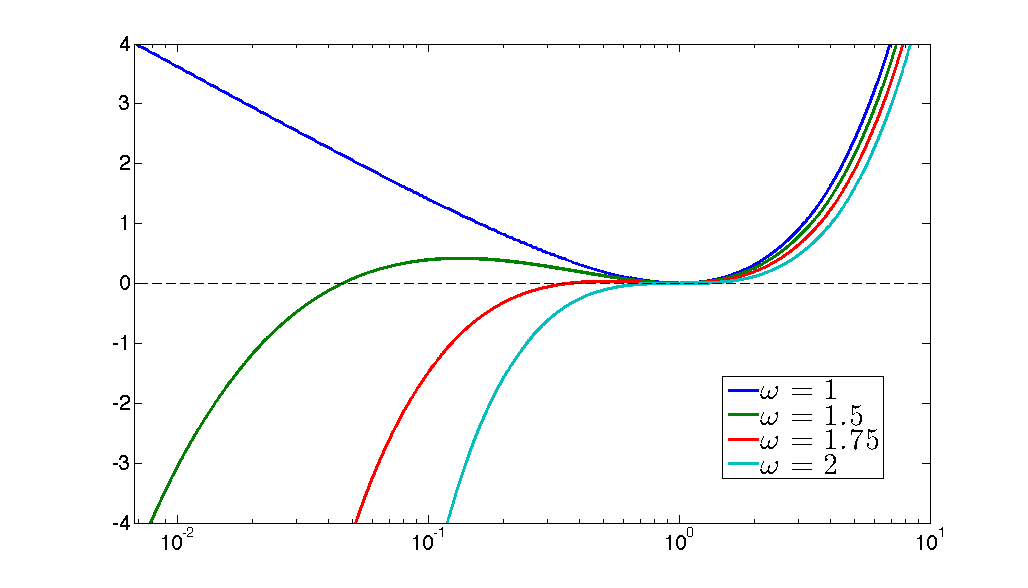
\includegraphics[width=11cm]{phi_omega.png}
\caption{\label{phi_omega} Plot of functions $\varphi_\omega(x)$ for different values $1\leq \omega\leq 2$ and   $x\in[10^{-2}, 10^1]$.}
\end{center}
\end{figure}
\subsection{Proposed algorithm}


\begin{theorem}\label{thm:algo}
	Take two continuous functions $\theta_1,\theta_2$ such that
	\begin{equation}\label{eq:cond_theta_k}
	\forall \gamma \in \IR_{+*}^{n_1 n_2},\quad
	F(P_{\Ccal_k}^{\theta_k(\gamma)}(\gamma)) \le F(\gamma) ,
	\end{equation}
	where the inequality is strict whenever $\gamma \notin \Ccal_k$.
	Consider the sequence defined by:
	\begin{align*}
	\gamma^0 &= e^{-c/\epsilon} \\
	\tilde{\gamma}^{l+1} &= P_{\Ccal_1}^{\theta_1(\gamma^l)}(\gamma^l) \\
	\gamma^{l+1} &= P_{\Ccal_2}^{\theta_2(\tilde{\gamma}^{l+1})}(\tilde{\gamma}^{l+1}).
	\end{align*}
	Then the sequence $(\gamma^l)$ converges to $\gamma^*$.
\end{theorem}

\begin{lemma}[]
	\label{lemma:trivial_intersection}
	Let us take $\gamma^0$ in $\IR_{+*}^{n_1 n_2}$,
	and denote
	\[
	S = \left\{
	\diag(a) \gamma^0 \diag(b),\quad
	(a,b) \in \IR_{+*}^{n_1 + n_2}
	\right\}
	\]
	the set of matrices that are diagonally similar to $\gamma^0$.
	Then the set $S \cap \Ccal_1 \cap \Ccal_2$ contains exactly one element $\gamma^* = P_{\Ccal_1 \cap \Ccal_2}(\gamma^0)$.
\end{lemma}
We refer to \cite{cuturi13} for the proof of this well-known result, which is used in the proof of the theorem.


\begin{proof}[Proof of the theorem]
	First of all, notice that the operators $P_{\Ccal_k}^\theta$ apply a scaling to lines or columns of matrices. All $(\gamma^l)$ are thus diagonally similar to $\gamma^0$:
	\[
	\forall l\ge0,\quad \gamma^l \in S
	\]
	
	By construction of the functions $\theta_k$, the sequence of values of the Lyapunov function $(F(\gamma^l))$ is non-increasing. Hence $(\gamma^l)$ is precompact.
	
	If $\xi$ is a cluster point of $(\gamma^l)$, let us define
	\begin{align*}
	\tilde{\xi} &= P_{\Ccal_1}^{\theta_1(\xi)}(\xi) \\
	\xi' &= P_{\Ccal_2}^{\theta_2(\tilde{\xi})}(\tilde{\xi}).
	\end{align*}
	Then by continuity of all the applications, $F(\xi) = F(\tilde{\xi}) = F(\xi')$.
	From the hypothesis made on $\theta_1$ and $\theta_2$, can be deduced that $\xi$ is in $\Ccal_1$ and that $\tilde{\xi}$ is in $\Ccal_2$. Therefore $\xi' = \tilde{\xi} = \xi$ is in the intersection $\Ccal_1 \cap \Ccal_2$.
	By lemma \ref{lemma:trivial_intersection}, $\xi = \gamma^*$, and the whole sequence $(\gamma^l)$ converges to the solution.
\end{proof}



%{\color{red} 
%	TODO Construire les bonnes fonctions $\theta_k(\gamma)$.}
To construct the functions $\theta_k$ needed by the theorem, we need the following lemma.

\begin{lemma}\label{lemma:F_P_theta}
	Let $1\le \theta < \omega$. Then, for any $\gamma \in \IR_{+*}^{nm}$, one has
	\begin{equation}\label{eq:F_P_theta}
	F(P^\theta_{\Ccal_k}(\gamma)) \le F(P^\omega_{\Ccal_k}(\gamma)).
	\end{equation}
	Moreover, equality occurs if and only if $\gamma \in \Ccal_k$.
\end{lemma}
\begin{proof}
	Thanks to lemma \ref{lemma:lyapunov_decrease}, one knows that
	\[
	F(P^\theta_{\Ccal_k}(\gamma)) - F(P^\omega_{\Ccal_k}(\gamma))
	= \scal{\mu^k}{(\varphi_\omega - \varphi_\theta) \left( \frac{A_k \gamma}{\mu^k} \right) } .
	\]
	Moreover, the function that maps $t \in [1,\infty)$ to $\varphi_t(x)$ is non-increasing:
	$\frac{d}{dt} \varphi_t(x) = \log x (x^{1-t} - 1).$
	For $x\neq 1$, it is even strictly decreasing.
	Thus the inequality (\ref{eq:F_P_theta}) is valid, with equality \emph{iff} $A_k \gamma = \mu^k$.
\end{proof}

\begin{proposition}
	We argue that a good choice for the functions $\theta_k$ may be constructed as follows. Pick a target parameter $\theta_0 \in [1;2)$, and a small $\delta>0$.
	Define the functions $\Theta^*$ and $\Theta$ as:
	\begin{align}
	\label{eq:Theta_opt}
	\Theta^*(u) &= \sup \left\{\omega \in [1;2]  \mid \varphi_\omega\left(\min u\right) \ge 0 \right\} ,\\
	\label{eq:Theta}
	\Theta(u) &= \min(\max(1,\Theta^*(u)-\delta),\theta_0),
	\end{align}
	where $\min u$ denotes the smallest coordinate of the vector $u$.
	Then the function
	\begin{equation}
	\label{eq:theta_k}
	\theta_k(\gamma) =\Theta\left (\frac{A_k \gamma}{\mu^k}\right)
	\end{equation}
	is continuous, and verifies condition (\ref{eq:cond_theta_k}).
\end{proposition}
This construction has several advantages.
One is that it allows to choose arbitrarily the parameter $\theta_0$ that will be used asymptotically. A heuristic for this choice is proposed in section \ref{section:local}.
But it is also an easy approach to having an adaptive method, as the approximation of $\theta_k^*$ has a negligible cost (it only require to solve a one dimensional problem that depends on the smallest value of $\frac{A_k \gamma}{\mu^k}$, and the corresponding function to invert is decreasing and concave).
We will show later on that this is often an excellent choice in practice.
\begin{proof}
	Since the partial derivative of $\frac{\partial\varphi_\omega(x)}{\partial\omega}$ is nonzero for any $x<1$, the implicit function theorem proves the continuity of $\Theta^*$.
	The function $\Theta^*\left(\frac{A_k \gamma}{\mu^k}\right)$ is such that every term in relation (\ref{eq:kl_diff_scal}) is non-negative.
	Therefore, by lemma \ref{lemma:F_P_theta}, using this parameter minus $\delta$ ensures the strong decrease (\ref{eq:cond_theta_k}) of the Lyapunov function.
	It is no problem to constrain it to $[1,\theta_0]$, as using 1 always verifies the inequality (\ref{eq:cond_theta_k}), and using $\theta_0$ when it is smaller than $\Theta^*\left(\frac{A_k \gamma}{\mu^k}\right)$ does as well.
\end{proof}

\section{Local rate of convergence ?}
\label{section:local}
Some material to adapt Lenaic results:


The SK algorithm can be interpreted as an alternate maximisation algorithm on the dual of the regularized optimal transport problem.
The dual problem of \eqref{ROT} is:
\begin{equation}\label{DROT}\max_{\alpha,\beta}\langle \alpha,\mu^1\rangle+\langle \beta,\mu^2\rangle-\epsilon\sum_{i,j}e^{(\alpha_i+\beta_j-c_{i,j})/\epsilon}\end{equation}
It is concave and continuously differentiable for all $(a,b)\in\IR^{n_1+n_2}$. Alternate maximization then converges and we recover, for $a_i=e^{\alpha_i/\epsilon}$, $b_j=e^{\beta_j/\epsilon}$ and $\gamma^0_{i,j}=e^{-c_{i,j}/\epsilon}$:
\begin{align*}
a^{l+1} &= {\mu^1}\oslash{\gamma^0 b^l} &
b^{l+1} &= {\mu^2}\oslash{^t \gamma^0 a^{l+1}} 
\end{align*}

If $(\alpha^*,\beta^*)$ is a solution of \eqref{DROT}, then all the 
other optimum can be written as $(\alpha^*+\kappa,\beta^*-\kappa)$, which means that the problem admits a unique solution, up to a translation with constant $\kappa\in\IR$.


The Hessian matrix of the functional in \eqref{DROT} at point $(\alpha,\beta)$ reads, for $a_i=e^{\alpha_i/\epsilon}>0$ and $b_j=e^{\beta_j/\epsilon}>0$:


$$H(a,b)=\frac1\epsilon\begin{bmatrix}
\diag(a)\diag(\gamma^0 b)&\diag(a)\gamma^0 \diag(b)\\
\diag(b){^t\gamma^0} \diag(a)&\diag(^t\gamma^0a)\diag(b)
\end{bmatrix}.$$
Notice that 

$$H(a^*,b^*)=\frac1\epsilon\begin{bmatrix}
\diag(\mu^1)&\gamma^*\\
^t\gamma^*&\diag(\mu^2)
\end{bmatrix}.$$


The matrices $H(a,b)$  are positive semi-definite. They have only one $0$ eigenvalue associated to the eigenvetor $^t[\mathbf{1},-\mathbf{1}]$. 
Using Schur complement properties, one can then show that any matrix $T(a,b)=(\diag(a)\diag(\gamma^0 b))^{-1}\diag(a)\gamma^0\diag(b)(\diag(^t\gamma^0a)\diag(b))^{-1} \diag(b){^t\gamma^0}\diag(a)=(\diag(\gamma^0 b))^{-1}\gamma^0(\diag(^t\gamma^0a))^{-1} \diag(b){^t\gamma^0}\diag(a)$ is positive semi definite for $a_i,b_j>0$. Moreover, we can show that $T$ has a unique largest eigenvalue that is $1$ and is associated to the eigenvector $\mathbf{1}$. All the other eigenvalues belongs to the set $[0;1[$.


From experiments, it seems possible to design a good guess for $\omega$ from $c$ and $\epsilon$ only. 
    Denoting as $\lambda$ the second larger eigenvalue of $T(1,1)$, one can set 
    $\omega=\frac{2}{\lambda}(1-\sqrt{1-\lambda})$.
    
    
    
\section{Experimental results}


%In practice, we observed that the algorithm introduced in Theorem \ref{thm:algo} can be simplified and it is sufficient to check $F(P^\omega_{\Ccal_2}(P^\omega_{\Ccal_1}(\gamma^l)))-F(\gamma^l)>0$ for performing the over-relaxed iterations with parameter $\omega$.
%The cost of this test is linear with respect to the data dimension (i.e. $o(n_1+n_2)$).

\renewcommand{\algorithmiccomment}[1]{\hfill\bgroup(#1)\egroup}
%\begin{algorithm}
%\caption{Over-relaxed SK algorithm}
%\label{SOR}
%\begin{algorithmic}
%\REQUIRE $\mu^1\in \IR^{n_1}$, $\mu^2\in \IR^{n_2}$, $c\in \IR^{n_1\times n_2}_+$
%\STATE Set $a=\mathbf{1}_{n_1}$, $b=\mathbf{1}_{n_2}$, $\gamma^0=e^{-c/\epsilon}$, $\omega\in[1;2[$ and $\eta>0$
%\WHILE {$||a\otimes \gamma^0b-  \mu_1||>\eta$}
%\STATE $\tilde a=\mu_1\oslash (\gamma^0 b)$,  $a_\omega=a^{1-\omega}\otimes \tilde a^\omega$
%\STATE $\tilde b=\mu_2\oslash (^t\gamma^0  a_\omega)$
%\IF{ $\langle \mu^1,\varphi_\omega(a\oslash\tilde a) \rangle +\langle \mu^2,\varphi_\omega(b\oslash\tilde b)\rangle>0$}
%\STATE  $a=a_\omega$, $b=b^{1-\omega}\otimes \tilde b^\omega$\COMMENT{Over-relaxed SK iteration}
%\ELSE
%\STATE $a=\tilde a$, $b=\mu_2\oslash (^t\gamma^0 a)$  \COMMENT{Sinkhorn iteration}
%\ENDIF
%\ENDWHILE
% \RETURN $\gamma=\diag(a)\gamma^0\diag(b)$
%\end{algorithmic}
%\end{algorithm}
Add algorithm to solve \eqref{eq:Theta_opt}?

This algorithm uses the function $\Theta$ defined in (\ref{eq:Theta}).

\begin{algorithm}
\caption{Over-relaxed SK algorithm }
\label{SOR}
\begin{algorithmic}
\REQUIRE $\mu^1\in \IR^{n_1}$, $\mu^2\in \IR^{n_2}$, $c\in \IR^{n_1\times n_2}_+$
\STATE Set $a=\mathbf{1}_{n_1}$, $b=\mathbf{1}_{n_2}$, $\gamma^0=e^{-c/\epsilon}$, $\theta_0\in[1;2)$ and $\eta>0$
\WHILE {$||a\otimes \gamma^0b-  \mu_1||>\eta$}
\STATE $\tilde a=\mu_1\oslash (\gamma^0 b)$, 
\STATE $\omega=\Theta(a\oslash\tilde a)$
%\IF{ $\langle \mu^1,\varphi_\omega(a\oslash\tilde a) \rangle>0$}
\STATE  $a=a^{1-\omega}\otimes \tilde a^\omega$%\COMMENT{Over-relaxed SK iteration}
%\ELSE
%\STATE $a=\tilde a$,\COMMENT{SK iteration}
%\ENDIF
\STATE $\tilde b=\mu_2\oslash (^t\gamma^0  a)$
\STATE $\omega=\Theta(b\oslash\tilde b)$
%\IF{ $\langle \mu^2,\varphi_\omega(b\oslash\tilde b) \rangle>0$}
\STATE  $b=b^{1-\omega}\otimes \tilde b^\omega$%\COMMENT{Over-relaxed SK iteration}
%\ELSE
%\STATE $b=\tilde b$,\COMMENT{SK iteration}
%\ENDIF
\ENDWHILE
 \RETURN $\gamma=\diag(a)\gamma^0\diag(b)$
\end{algorithmic}
\end{algorithm}



{\color{red} TODO}


\section{Conclusion and perspectives}

We have presented a generalization of the Sinkhorn--Knopp algorithm based on over-relaxed projections, with a criterion for global convergence based on a Lyapunov function.
The proposed Lyapunov function allows for an adaptive choice of over-relaxation parameter at a low computational price.
In practice, this algorithm converges way faster than Sinkhorn--Knopp; moreover, the acceleration rate is especially impressive for small regularization $\epsilon$.


Contributions: 
cheap test, preliminary work for convergence results. Huge acceleration in practice.


Perspectives:
global convergence, how chosing $\omega$?, intensive numerical study with respect to other accelerarions methods\cite{2016arXiv160604133S,2017arXiv170509634A}.

Links with monotone Fista? (that choose Fista if energy decreased and forward backward otherwise...)





\section*{Acknowledgments}
This study has been carried out with financial support from the French State, managed by the French National Research Agency (ANR) in the frame of the  GOTMI project (ANR-16-CE33-0010-01).

%\subsubsection*{References}

\bibliographystyle{apalike}
\bibliography{references}

\end{document}
